% Tento soubor nahraďte vlastním souborem s obsahem práce.
%=========================================================================
% Autoři: Michal Bidlo, Bohuslav Křena, Jaroslav Dytrych, Petr Veigend a Adam Herout 2019

% Pro kompilaci po částech (viz projekt.tex), nutno odkomentovat a upravit
%\documentclass[../projekt.tex]{subfiles}
%\begin{document}

\chapter{Úvod}
Tato práce se zabývá tematikou robotiky. Primárním zaměřením je systém pro řízení robotů jménem Robot Operating System 2. ROS2, jak z názvu vyplývá, je již druhá verze těchto nástrojů. V minulosti se originální ROS stal de facto standardem pro vývoj softwaru k~řízení robotů. Většina práce řeší softwarovou stranu této problematiky. Obor robotiky jako takový se však pohybuje velice blízko hardwaru, a tak se tato práce dotýká také některých hardwarových konceptů a principů potřebných k pochopení použitých komponent.

Jak už bylo zmíněno, zaměřením práce je samotný ROS2. Jádro práce se tedy snaží demonstrovat funkcionalitu a možnosti tohoto middleware. Obsahem této části je tvorba systému, který bude využívat nástroje ROS2 k ovládání robota. Jako hardware, nad kterým bude celá práce implementována, byla zvolena stavebnice Adeept AWR 4WD. Kromě čistého ROS2 se práce zaměřuje také na související nástroje a systémy, které nějakým způsobem využívají nebo rozšiřují funkcionalitu ROS2. Prvním z nich je knihovna ros2\_control, která slouží k řízení pohybu robotů. Jako druhé, práce demonstruje použití Gazebo simulátoru pro vývoj a testování robotického softwaru. Posledním rozšířením je přidání lidar senzoru pro mapování a navigaci robota v prostoru.

První polovina této dokumentace se zaměřuje na vysvětlení teoretičtějších konceptů souvisejících s danou problematikou. Nejprve se představuje použitý hardware a principy fungování jednotlivých komponent. Následně přechází na samotný ROS2. Tato část se nejprve podívá na to, co ROS2 vlastně je a jak vnitřně funguje. Následně jsou vysvětleny koncepty, které používají vývojáři při interakci a vývoji ROS2 systému. Konec teoretické části se zaměřuje na rozšíření.
Obsahem druhé poloviny je představení vytvořeného ROS2 systému. Prakticky ukazuje využití jednotlivých ROS2 funkcionalit. Tato polovina je také rozdělena na dvě části. Ta první se zaměří na možnosti čistého ROS2. Probírají se zde jednotlivé uzly pro ovládání hardwaru, ale také uzly pro řízení robota jako celku. Druhá část se zaměří na obohacení tohoto systému o další související nástroje. Jejím obsahem je zprovoznění těchto nástrojů a následné propojení s ROS2.

\chapter{Použitý Hardware}
ROS2 je nástroj sloužící k tvorbě robotických aplikací. Z toho důvodu je k demonstraci jeho možností vyžadováno použití nějakého fyzického robota, nad kterým bude aplikace implementována. V této práci byl jako demonstrační robot použit Adeept AWR 4WD. Z~této stavebnice pochází většina komponentů. V pozdější fázi byl tento základ rozšířen o~další hardware. Ten byl následně použit k demonstraci pokročilejších konceptů. Mozkem robota je mikropočítač Raspberry Pi 4.

\section{Hardwarové technologie}
V první sekci budou představeny obecné hardwarové technologie. Jedná se o relativně známé koncepty. V souvislosti této práce je využívají některé z použitých komponent.

\subsection*{Pulzně šířková modulace} 
Umožňuje vytvořit pseudo-analogový výstupní signál na číslicových pinech mikrokontroléru. Mikrokontroléry jsou digitální zařízení a chtěly by tedy s okolním světem komunikovat pomocí jedniček a nul. Reálný svět tak ovšem nefunguje, a proto je často potřeba převádět výstup z mikrokontroléru na analogový signál. Problém je v tom, že převod digitálního signálu na analogový je relativně dlouhá a neefektivní operace. Proto vznikla pulzně šířková modulace (PWM), která umožňuje simulovat analogový výstup.

PWM využívá toho, že člověk nedokáže rozpoznat rychlé změny. Příkladem může být led dioda blikající na frekvenci 5000 Hz. Člověku se jeví, jako by svítila permanentně. Mechanická zařízení to mají podobně. Pokud je PWM generováno na dostatečně vysoké frekvenci, tak z pohledu stejnosměrného motoru se může zdát, že dostává konstantní analogové napájení.

\begin{figure}[h!]
	\centering
	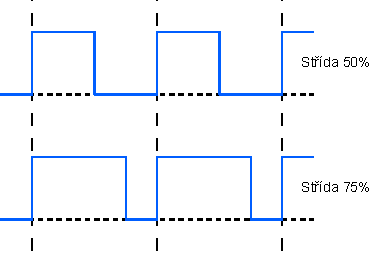
\includegraphics[scale=1.2]{obrazky-figures/pwm_duty_cycle.pdf}
	\caption{PWM signál pro různé hodnoty střídy}
	\label{fig:pwm}
\end{figure}

\newpage
Při pohledu na klasický digitální signál (obr:~\ref{fig:pwm}), který rovnoměrně střídá vysokou a nízkou úroveň, by šlo říci, že se jedná o PWM signál se střídou 50\%. Střída (duty cycle) udává poměr času, kdy je signál v logické jedničce, ku času, kdy je v nule. Součet těchto hodnot se musí rovnat délce jedné periody. Úpravou tohoto poměru lze simulovat analogový \\ signál.~\cite[str:~116-118]{embeded_robotics}

\subsection*{I2C}
Je synchronní sběrnice, která se vyznačuje svou jednoduchostí a nízkou cenou. Využívá dva vodiče SDA (serial data) a SCL (serial clock). Oba vodiče jsou připojeny k napájecímu napětí pomocí pull-up rezistoru. Bez vlivu jiného hardwaru zůstává jejich logická hodnota v~jedničce. Zařízení, která jsou na tuto sběrnici připojeny, využívají open drain (obr:~\ref{fig:open_drain}) k úpravě aktuální napěťové úrovně. I2C pracuje s dvěma druhy zařízení, master a slave. Master zahajuje, řídí a ukončuje komunikaci na vodiči SDA. Po dobu komunikace také generuje hodinový signál na SCL. Typicky se jedná o mikrokontrolér. Za slave se označují ostatní zařízení, s nimiž může master komunikovat. Typicky to jsou různé periferie. \cite[str:~88]{embeded_robotics}

\begin{figure}[h!]
	\centering
	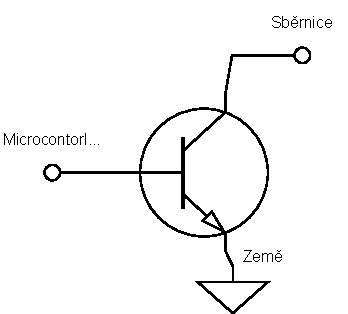
\includegraphics[scale=1]{obrazky-figures/open_drain.pdf}
	\caption{Open drain}
	\label{fig:open_drain}
\end{figure}

Přenos datového rámce zahájí master zařízení přivedením datové sběrnice do nuly. Následující komunikace se skládá z odeslání rámce o délce osmi bitů a potvrzení o úspěšném přenosu dat od přijímajícího zařízení. Toto potvrzení se nazývá ACK a je provedeno podržením datové sběrnice v hodnotě nula po dobu jednoho taktu. Opačný stav se nazývá NACK a indikuje že nastala chyba. Ukončení přenosu je provedeno navrácením datové sběrnice na hodnotu jedna. \cite[str:~8-10]{um10204}

\begin{figure}[h!]
	\centering
	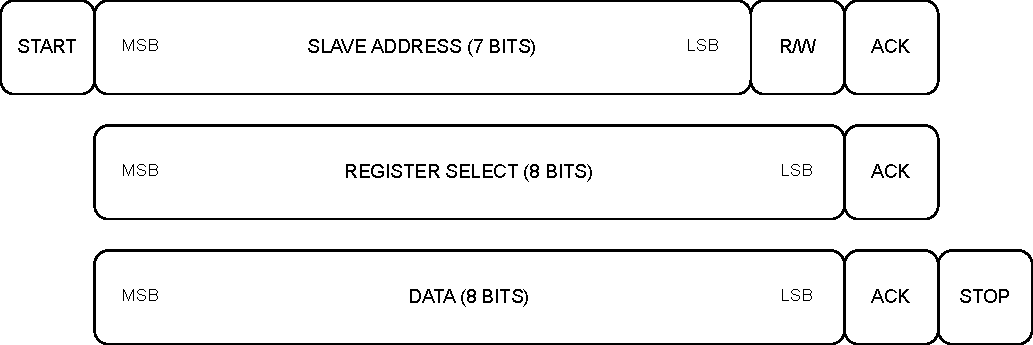
\includegraphics[scale=0.75]{obrazky-figures/i2c_data_word.pdf}
	\caption{Datové slovo sběrnice I2C}
	\label{fig:i2c_word}
\end{figure}

Na obrázku \ref{fig:i2c_word} lze vidět, jak může vypadat přenos jednoho datového slova. V prvním rámci je přenesena sedmi bitová adresa, identifikující slave zařízení, se kterým chce master navázat komunikaci. Osmý bit datového rámce indikuje směr, kterým budou posílány data. V druhém rámci dojde k adresaci konkrétního registru na slave zařízení. A ve třetím, případně dalších, již probíhá samotné posílání dat mezi zařízeními. \cite[str:~88]{embeded_robotics}

\section{Adeept AWR 4WD}
Tato sekce se již zaměří na použitého robota (obr:~\ref{fig:robot}). Následující stránky postupně představují jeho komponenty. Cílem je ukázat schopnosti robota a vysvětlit princip fungování těchto součástek.\footnote{\url{https://www.adeept.com/awr_p0122.html}}

\begin{figure}[h!]
	\centering
	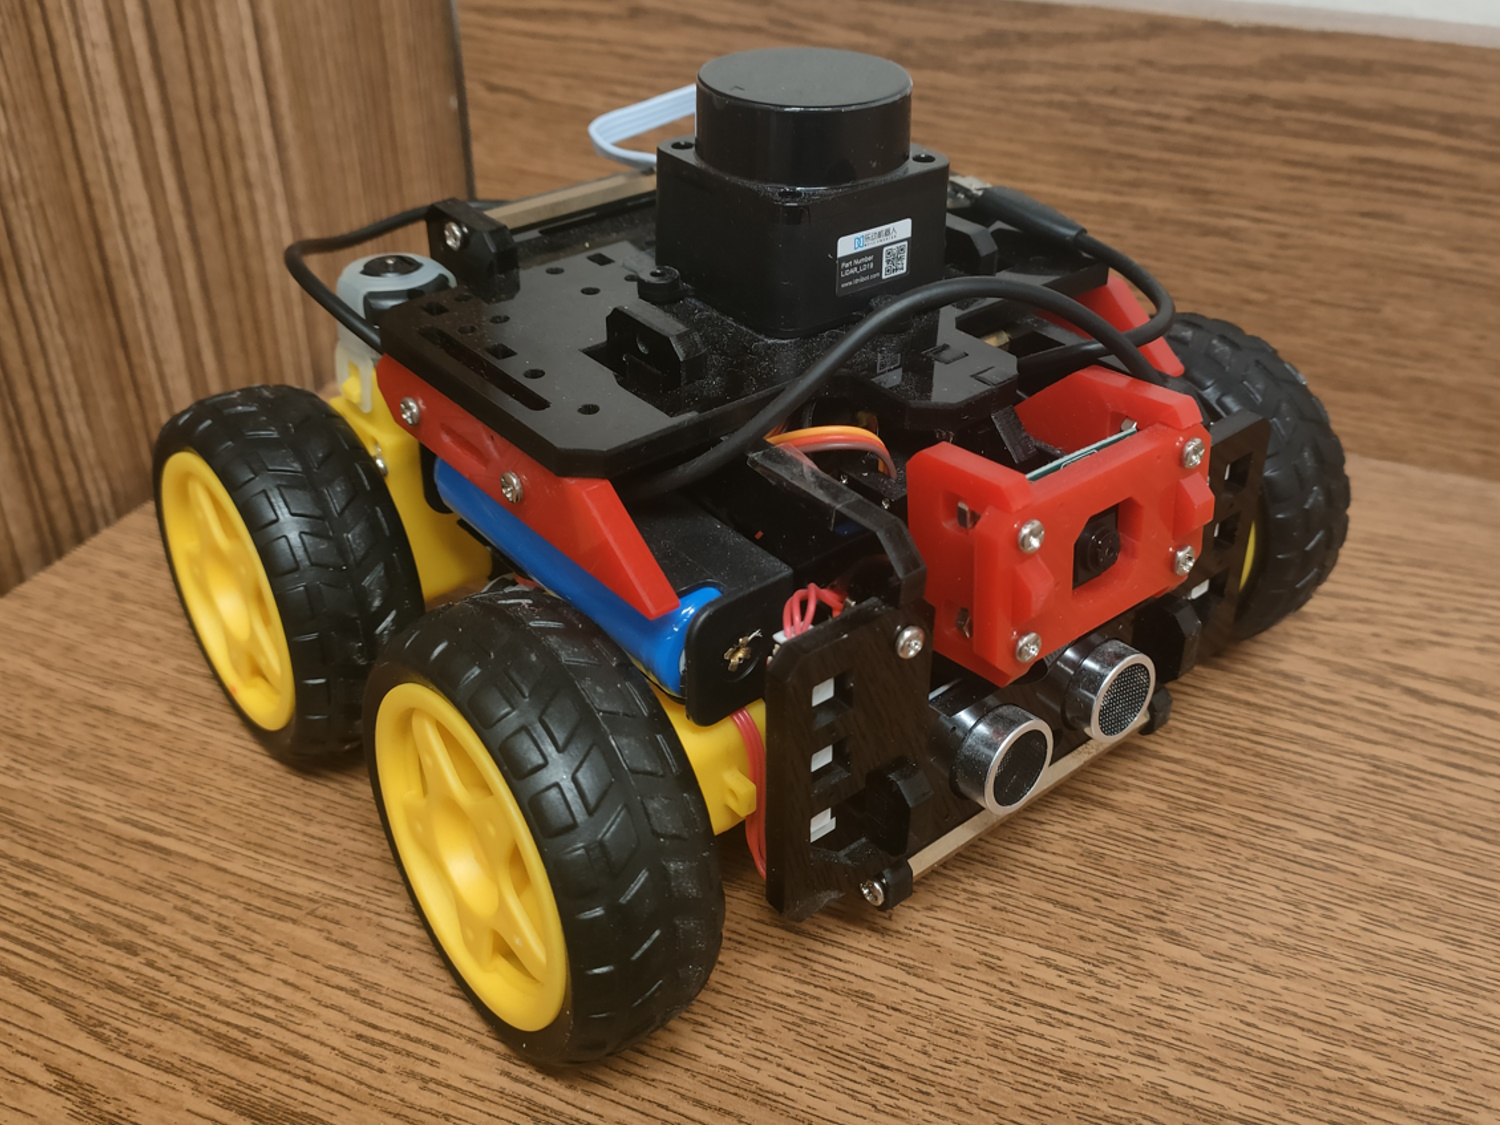
\includegraphics[scale=0.2]{obrazky-figures/robot.jpg}
	\caption{Robot Adeept AWR 4WD s rozšířeními}
	\label{fig:robot}
\end{figure}

\subsection*{Robot HAT}
HAT (hardware attached on top) je hardwarová deska, která slouží k rozšíření funkcionality mikrokontroléru. Tato konkrétní, se k Raspberry Pi připojuje pomocí GPIO (general purpose input output) pinů. Deska jako taková obsahuje rozšiřující čipy a rozhraní sloužící k ovládání připojených periferií.

\newpage
\begin{itemize}
	\item{PCA9685 \cite[str:~2]{pca9685}}
	\begin{itemize}
		\item{generátor PWM signálu}
		\item{16 kanálů}
		\item{střída s rozlišením 12 bitů(4096 možných hodnot)}
		\item{ovládání přes I2C sběrnici}
	\end{itemize}
	\item{L298P \cite{l298}}
	\begin{itemize}
		\item{ovladač pro řízení dc motoru}
		\item{základem je full bridge obvod, obr:~\ref{fig:full_bridge}}
		\item{umožňuje roztočit motor oběma směry}
		\item{pomocí PWM lze ovládat rychlost motorů}
		\item{připojuje motor na externí napájení}
	\end{itemize}
	\item{další rozhraní pro připojení periferií (sledování čáry, ultrazvukový senzor, led)}
\end{itemize}

\begin{figure}[h!]
	\centering
	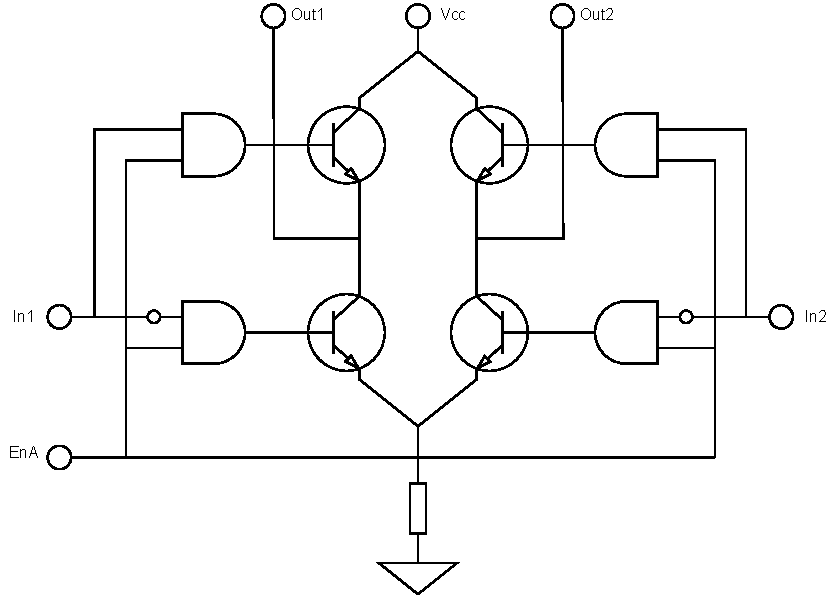
\includegraphics[scale=0.75]{obrazky-figures/motor_full_bridge.pdf}
	\caption[Full bridge zapojení ovladače stejnosměrných motorů]{Full bridge konfigurace pro ovládání motoru. In1 a In2 určují směr otáčení. EnA je PWM signál určující rychlost otáčení. \cite[str:~1]{l298}}
	\label{fig:full_bridge}
\end{figure}

\subsection*{Stejnosměrný motor}
Pohyb celého autíčka zajišťují čtyři stejnosměrným proudem (direct current) napájené motory. Ovladač motorů L298P je umístěný na Robot HAT.

\begin{figure}[h!]
	\centering
	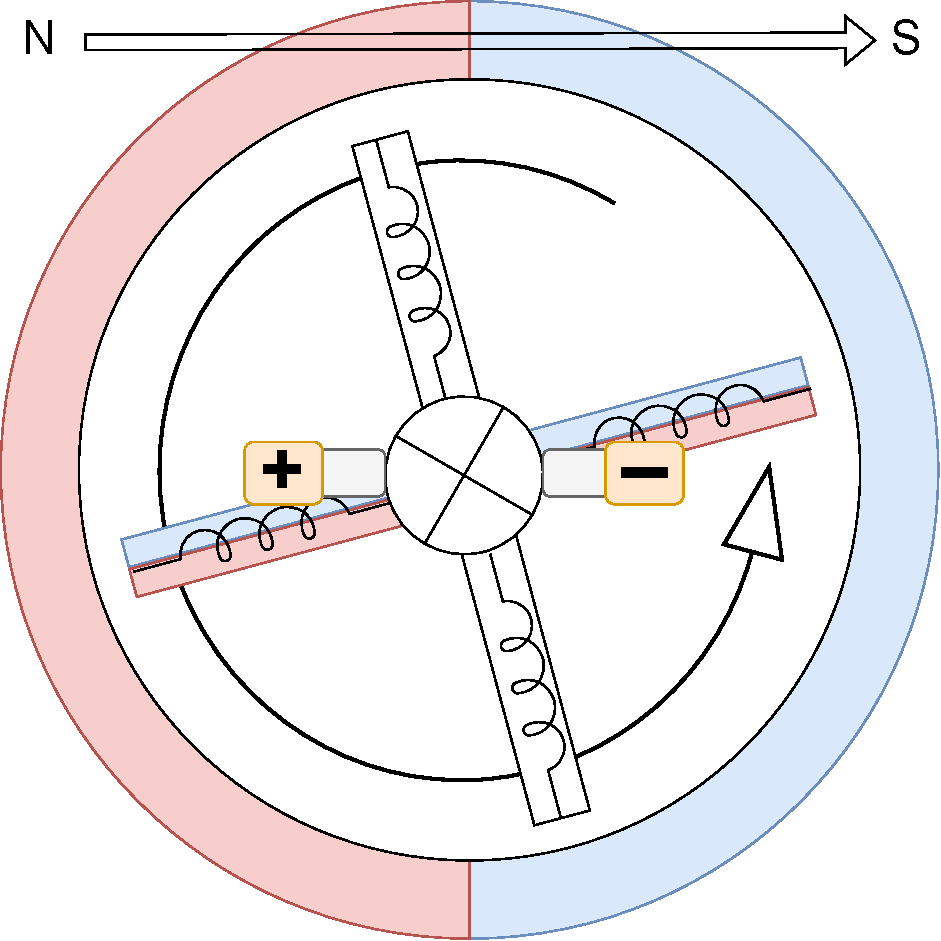
\includegraphics[scale=0.5]{obrazky-figures/dc_motor.pdf}
	\caption{Schéma DC motoru}
	\label{fig:dc_motor}
\end{figure}

Elektrický DC motor (obr:~\ref{fig:dc_motor}) se skládá ze dvou hlavních částí, stator a rotor. Stator je statická vnější část a typicky se jedná o permanentní magnet. Uvnitř statoru se nachází rotor. Ten je tvořen několika elektromagnety. V momentě jejich zapnutí dojde k reakci se statorem (opačné póly se přitahují a stejné odpuzují) a hřídel motoru se tak částečně pootočí. Při správném spínání a vypínání elektromagnetů lze motor rozběhnout.
Toto střídání zajišťuje prstenec zvaný komutátor. Komutátor je rozdělen na několik od sebe odizolovaných částí, ke kterým jsou připojeny vývody elektromagnetů. S povrchem prstence jsou pomocí pružin v kontaktu dva kartáče. Tyto kartáče se již neotáčí a mohou tak být připojeny na zdroj napájení a zem. Komutátor se otáčí společně s rotorem a při tomto pohybu se kartáče postupně dotýkají různých částí komutátoru a spínají tak jednotlivé elektromagnety. Ty zajistí pootočení rotoru a sepnutí následujícího magnetu. \cite[std:~28-36]{mobilní_roboty}

\subsubsection{Robot s diferenciálním podvozkem}
Tento konkrétní robot disponuje čtyřmi motory. Ty jsou pevně připevněny k tělu robota. Z toho důvodu je zatáčení realizováno diferenciálním způsobem. Tento přístup využívá toho, že motory nejsou na sobě navzájem závislé a můžou se tedy otáčet různými rychlostmi. Pokud se kola na jedné straně robota otáčejí rychleji, urazí větší vzdálenost. Z~toho pak vyplývá, že výsledné trajektorie již nejsou dvě rovnoběžky, ale soustředné kružnice. V porovnání s ostatními přístupy pro realizaci pohybu robota se jedná o konstrukčně jednodušší řešení, protože nevyžaduje natáčení kol do stran. Další výhodou je možnost otáčení robota na místě. \cite[str:~5]{embeded_robotics}

\subsection*{Servo}
Servo je komponenta, která se na první pohled velmi podobá stejnosměrnému motoru. Rozdílem je fakt, že se neotáčí donekonečna, ale bývá omezena nějakým úhlem (například 180 stupňů). Hlavní výhodou a důvodem pro použití serva je plná kontrola nad úhlem natočení jeho hřídele. \cite[str:~119-121]{embeded_robotics}

\begin{figure}[h!]
	\centering
	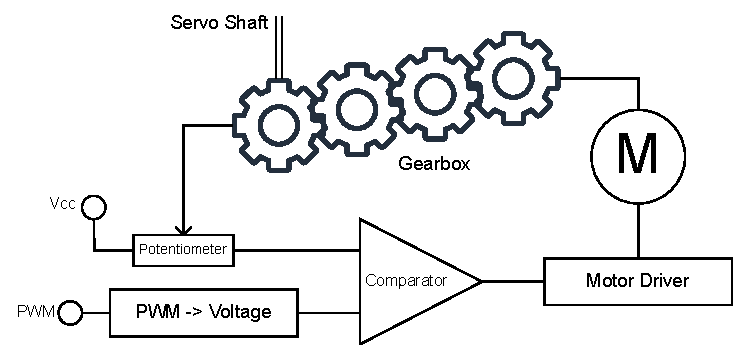
\includegraphics[scale=0.9]{obrazky-figures/servo.pdf}
	\caption{Vnitřní zapojení serva}
	\label{fig:servo}
\end{figure}

Při pohledu na vnitřní zapojení serva (obr:~\ref{fig:servo}) lze zjistit, že jádrem je opravdu klasický stejnosměrný motor. Není však jedinou částí. Dále servo obsahuje převodovku a řídící elektroniku. K nastavení výsledného úhlu serva se používá PWM signál. Ten je nejprve přeložen na napěťovou úroveň. Získaná hodnota je porovnána s aktuálním natočením serva a výsledek udává směr, kterým se bude motor otáčet. Aktuální úhel serva je získán z potenciometru zapojeného na výstupní hřídel serva. \cite[str:~89-90]{mobilní_roboty}

\subsection*{Ultrazvukový senzor hloubky} \label{theory:ultrasonic}
V podstatě se jedná o sonar (obr:~\ref{fig:ultrasonic}). Slouží k určení vzdálenosti. Senzor zahajuje měření po přijetí signálu na trig pinu. Následně je odesláno 8 ultrazvukových pulzů na frekvenci 40~Hz. Výsledkem měření je časový interval mezi odesláním pulzu a přijetím ozvěny. Tato informace se předává zpět mikrokontroléru. To je provedeno nastavením echo pinu do hodnoty jedna na dobu rovnou výsledku měření. \cite[str:~93]{embeded_robotics}

\begin{figure}[h!]
	\centering
	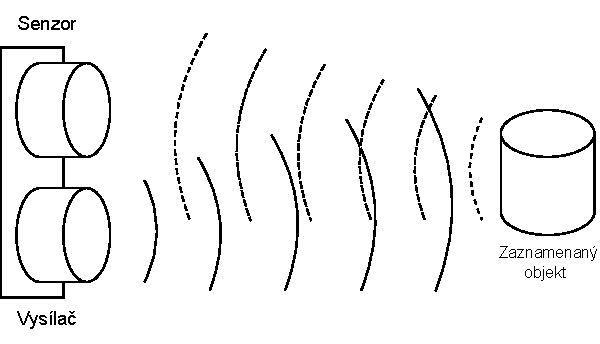
\includegraphics[scale=0.75]{obrazky-figures/ultrasonic.pdf}
	\caption{Ultrazvukový senzor}
	\label{fig:ultrasonic}
\end{figure}

Pro výpočet vzdálenosti lze využít následující vzorec:

\begin{equation}
	S = \frac{(T_2 - T_1) * V_S}{2}
\end{equation}

Kde $T_1$ je moment vyslání pulzu, $T_2$ moment zachycení ozvěny a $V_S$ rychlost šíření zvuku ve vzduchu (cca 340 m/s). Výsledek se pak dělí dvěma, protože doba $T_2 - T_1$ je rovna času k překážce a zpět. \cite[str:~132]{mobilní_roboty}

\newpage
\subsection*{Třícestný senzor pro sledování čáry}
Modul používá tři stejné senzory. Skládají se z infračervené diody a snímače odraženého světla. Jedná se o levnější verzi laserových senzorů používaných k měření vzdálenosti. Na rozdíl od nich jsou osazeny pouze infračervenou diodou, která má výrazně menší dosah. Typickým použitím podobných senzorů je detekce blízkosti k překážce (proximity sensor). Kromě toho, že tyto senzory nemají velký dosah, jsou jejich hodnoty ovlivněny také barvou a materiálem povrchu, od kterého se světlo odráží. A přesně to využívá modul pro sledování čáry. Světlý povrch odráží výrazně více světla než černý. Senzory tak hlídají množství přijatého světla a podle toho nastavují své výstupy. Přímo na modulu je umístěn potenciometr pro nastavení citlivosti všech tří senzorů. \cite[str:~115, 148]{mobilní_roboty}

\subsection*{WS2812 RGB LED}
V nejjednodušším případě jsou diody k mikrokontroléru připojeny napřímo pomocí GPIO pinů. Při použití většího počtu ledek se tento přístup stává nepoužitelným. Jedním z řešení je použití WS2812. Jedná se o druh adresovatelných led diod. Tento přistup umožňuje připojit několik set diod pomocí pouze tří vodičů. Konkrétně je použit jeden datový vodič, napájení a země. \cite[str:~2]{ws2812}

\begin{figure}[h!]
	\centering
	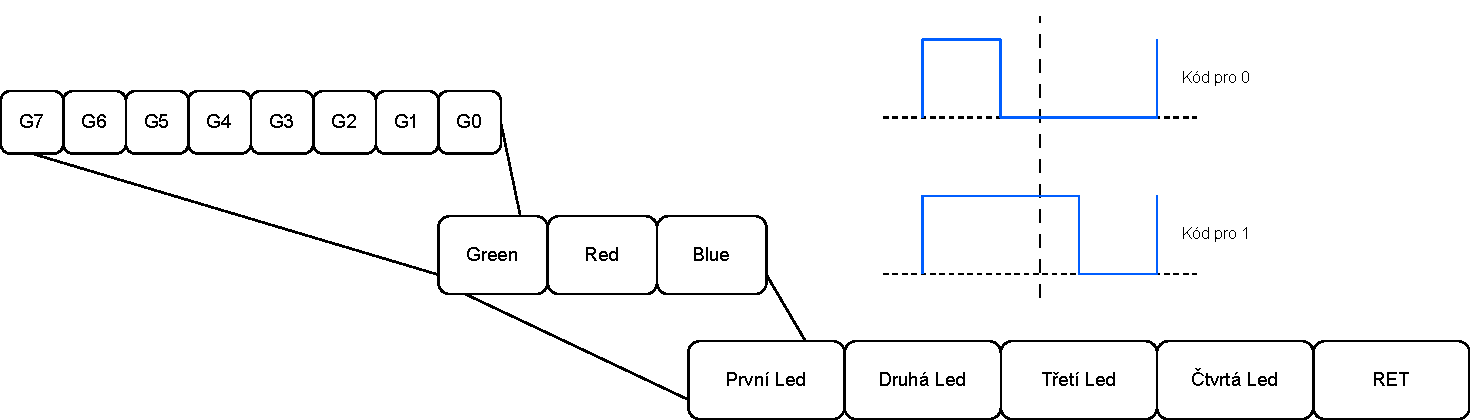
\includegraphics[scale=0.6]{obrazky-figures/ws2812_led.pdf}
	\caption{Komunikační protokol pro WS2812 led}
	\label{fig:ws2812_protocol}
\end{figure}

Diody jsou na pásku zapojeny sériově. Každá dioda má DIN a DO port. Komunikace (obr:~\ref{fig:ws2812_protocol}) vždy začíná klidovým stavem (datový vodič je v nule). Datové slovo se skládá z~24bitových bloků. Jeden pro každou diodu. Blok obsahuje tři osmi bitové hodnoty. Jednu pro každou barevnou složku (MSB je posíláno první). Diody pak fungují tak, že přijmou prvních 24 bitů, podle kterých nastaví svou barvu. Tuto část odeberou z datového slova a~zbytek přeposílají na výstup. \cite[str:~4]{ws2812}

\section{Rozšiřující komponenty}
V minulé sekci byly představeny komponenty, které jsou součástí Adeept kitu. V průběhu vývoje ROS2 systému se objevovaly požadavky na další rozšíření, které by dokázaly vylepšit výsledný produkt. Proto bylo originální hardwarové vybavení doplněno o následující komponenty.

\subsection*{Inertial measurement unit}
Jedná se o druh senzoru, jehož úkolem je určení orientace a pozice v prostoru. Použitý IMU disponuje třemi senzory. Pro měření rotace je obsazen tříosým gyroskopem. Pro určení zrychlení, případně rychlosti, disponuje také tříosým akcelerometrem. Poslední funkcí tohoto senzoru je ještě zabudovaný teploměr. Ten však není v této práci použitý.

\subsubsection*{MEMS}
Pod pojmem gyroskop si snad každý představí mechanickou rotující součástku, která udržuje svou orientaci. Tento přístup však nelze použít na miniaturních čipech IMU senzorů. MEMS je zkratka pro micro-electromechanical systems. Jak z názvu vyplývá jedná se o~systémy využívající mechanické elementy ve velikostech typických pro elektronické součástky.~\cite[str:~2-3]{mems_acc}

\subsubsection*{Princip akcelerometru}
Následující obrázek \ref{fig:mems_acc} zobrazuje vnitřní strukturu akcelerometru. Senzor se skládá ze dvou hlavních částí. Tou první je pohyblivé oranžové závaží. Protože má nezanedbatelnou hmotnost, je ovlivněno vnějšími vlivy. V případě, že se změní akcelerace působící na senzor, dojde také ke změně relativní pozice mezi tímto závažím a zbytkem senzoru. Tento pohyb je měřen a určuje výslednou akceleraci. Obě části obsahují desky, které tvoří části kondenzátorů. Při pohybu vnitřní části, dojde ke změně vzdálenosti mezi deskami, a tedy i změně kapacity kondenzátorů. Podrobněji viz \cite[str:~4-5]{mems_acc}

\begin{figure}[h!]
	\centering
	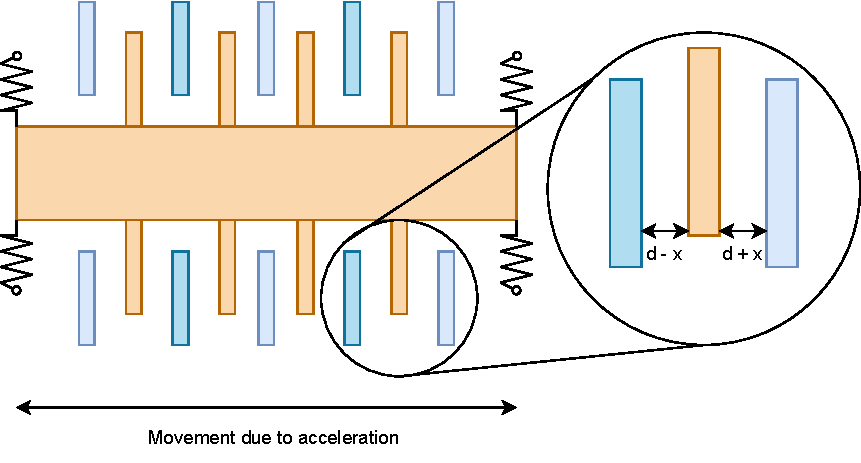
\includegraphics[scale=0.8]{obrazky-figures/accelerometer.pdf}
	\caption{Vnitřní struktura MEMS akcelerometru}
	\label{fig:mems_acc}
\end{figure}

\subsubsection{Princip gyroskopu}
MEMS gyroskop (obr:~\ref{fig:mems_gyro}) využívá podobné principy jako akcelerometr. Skládá se ze dvou částí, vnitřní rám a senzorický rám. Ve vnitřním rámu je umístěno pohyblivé závaží. Na rozdíl od akcelerometru není tato část v klidovém stavu statická, ale je rozvibrována do harmonické oscilace podél osy x.
Vnitřní rám je celý umístěn pohyblivě, uvnitř senzorického rámu. Když potom dojde k rotaci senzoru, bude vnitřní oscilující část držet svůj původní směr. To způsobí pohyb vnitřního rámu podél osy y. Vnější a vnitřní rámy jsou stejně jako u~akcelerometru obsazeny deskami kondenzátorů. Změna v jejich kapacitě je opět hlídána a~přepočítána na rotaci. \cite{mems_gyro}

\begin{figure}[h!]
	\centering
	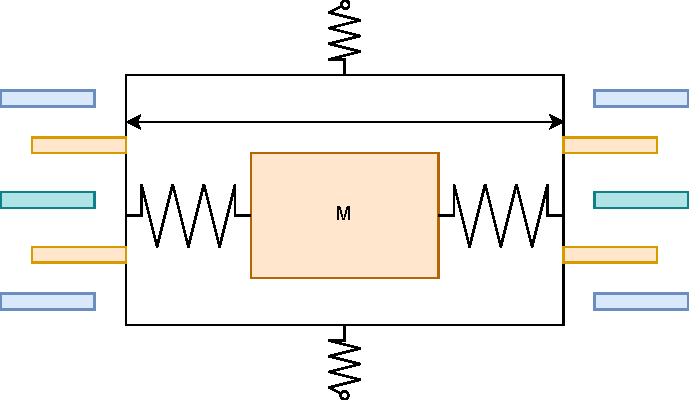
\includegraphics[scale=0.8]{obrazky-figures/gyroscope.pdf}
	\caption{Vnitřní struktura MEMS gyroskopu}
	\label{fig:mems_gyro}
\end{figure}

\newpage
\subsection*{Light detection and ranging}
Principiálně je lidar podobný ultrazvukovému senzoru. Hlavním rozdílem je to, že lidar používá pro měření laser. Data získaná lidarem tak bývají z pravidla přesnější oproti sonaru. Hlavní důvod přidání lidaru však není jeho vyšší přesnost. Tento konkrétní model totiž umožňuje měření v celých 360° okolo robota. Díky tomu lze data získaná z tohoto senzoru použít k mapování a lokalizaci robota v prostoru. \cite[str:~96-98]{embeded_robotics}

\begin{figure}[h!]
	\centering
	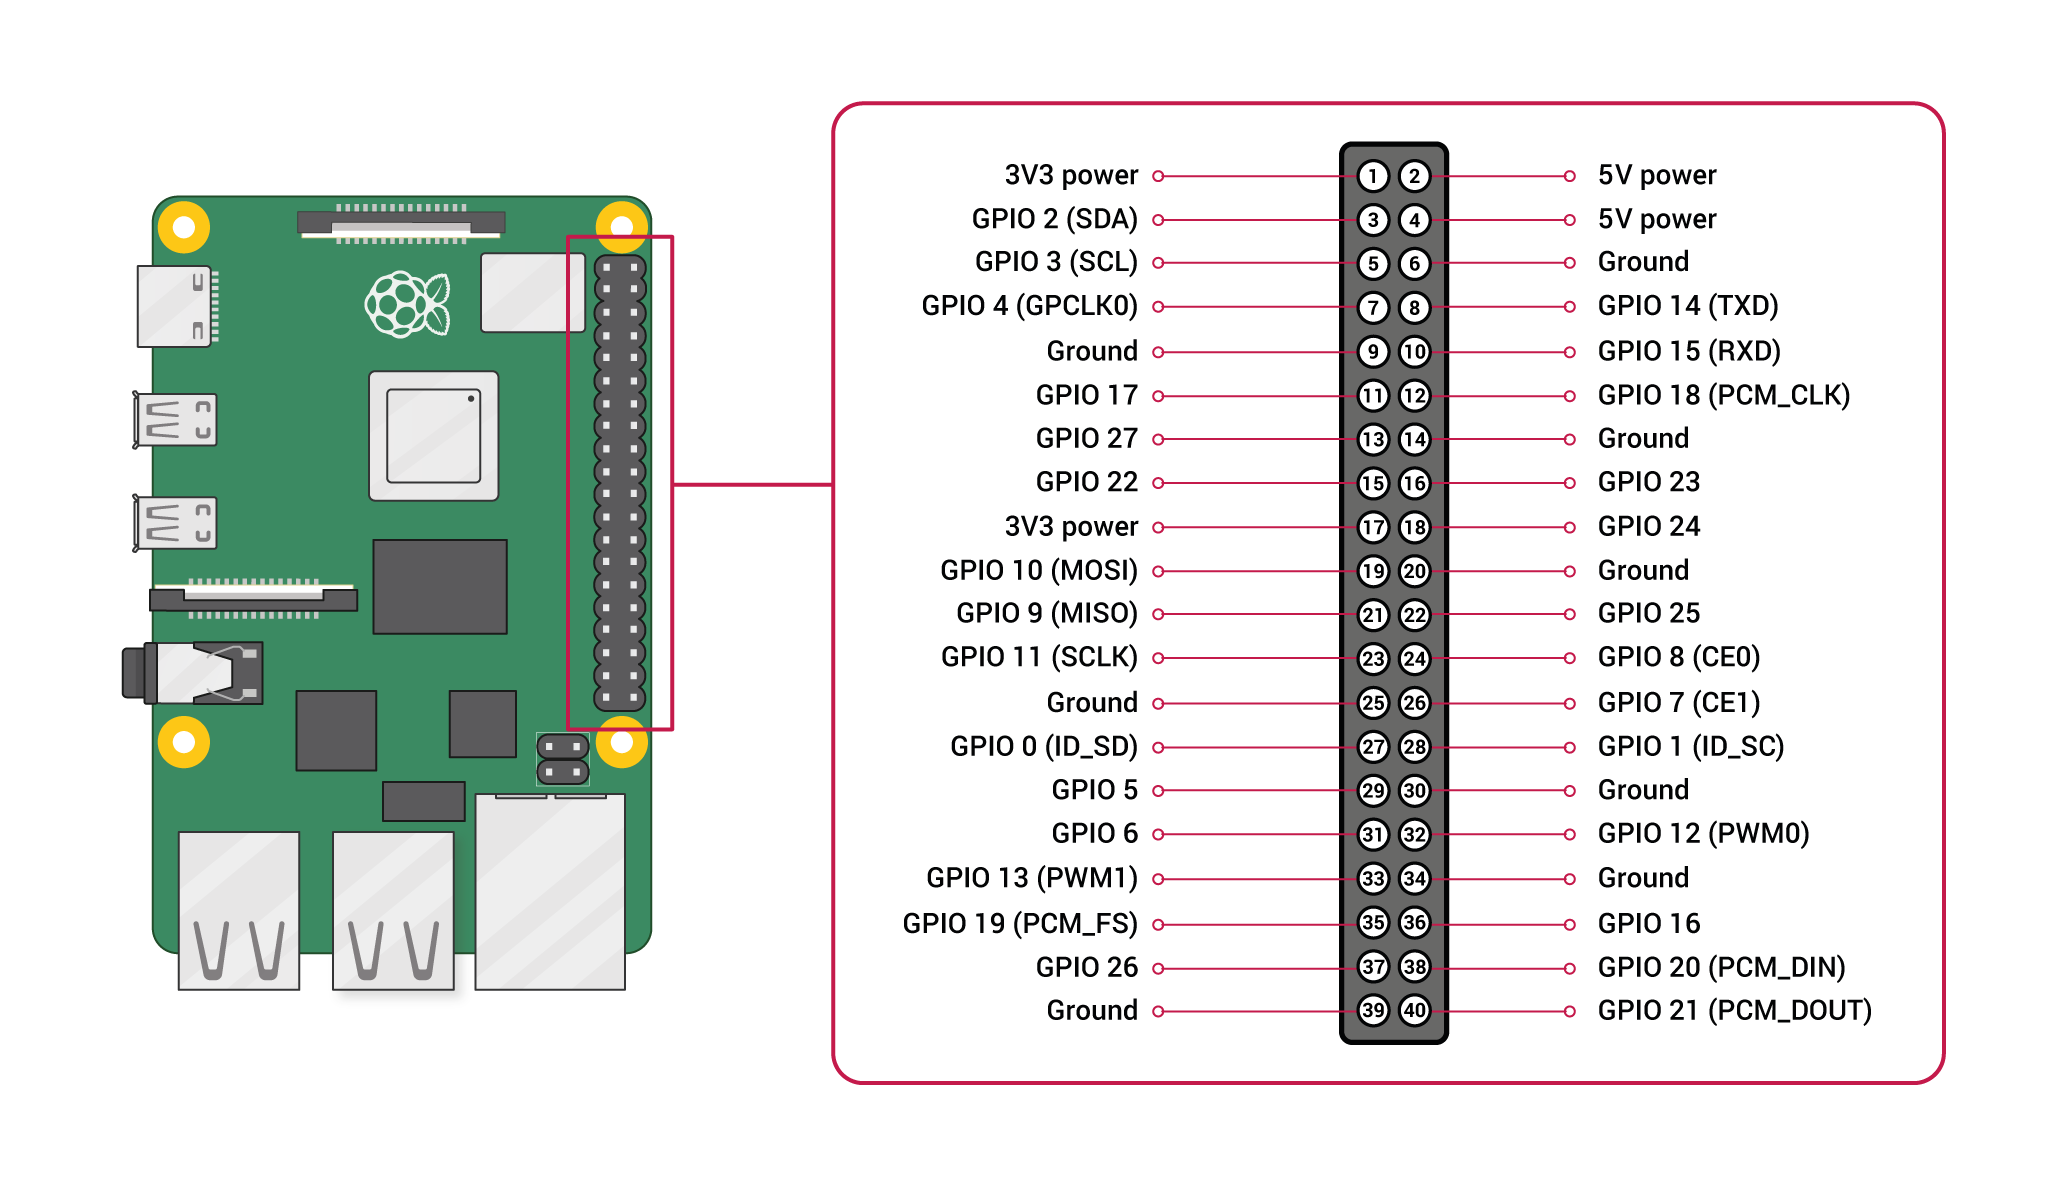
\includegraphics[scale=0.15]{obrazky-figures/gpio_pinout.png}
	\caption[GPIO pinout pro Raspberry Pi]{GPIO pinout pro Raspberry Pi, převzato z \cite{rpi_documentation}}
	\label{fig:rpi_gpio_pinout}
\end{figure}

\section{Raspberry Pi 4B}
Jako mozek celého systému je použit mikropočítač Raspberry Pi. Konkrétně verzi~4 model~B s~operační pamětí o velikosti čtyř gigabajtů. Tato verze disponuje 64bitovým procesorem, který je potřeba pro spuštění 64bitového Ubuntu serveru. Jedná se o doporučený operační systém pro běh ROS2 na platformě Raspberry Pi.
Komunikace s většinou použitých periferií je uskutečněna pomocí GPIO pinů (obr:~\ref{fig:rpi_gpio_pinout}). GPIO jsou číslicové vývody, které podle potřeby můžou fungovat jako vstup i výstup ze zařízení. Některé z nich pak mají ještě speciální funkce, například GPIO 2 a 3 můžou pracovat jako SDA a SCL připojení pro I2C komunikaci. \cite{rpi_documentation}

\subsection*{Kamera}
Přímo k Raspberry Pi je připojen oficiální Camera Module 3. Tento modul dokáže nahrávat video až v rozlišení 2304 × 1296 pixelů a 56 snímcích za vteřinu. \cite{rpi_documentation}

\chapter{Robot Operating System 2}
Tato kapitola slouží k představení ROS2. Začátek se zaměří na vnitřní fungování systému. Následně budou představeny koncepty, na kterých je ROS2 postavený a které jsou potřebné pro vývoj aplikací používajících tento middleware. Závěr této kapitoly pak projde další části ROS2 jako nástroje příkazové řádky, spouštění uzlů a transformační subsystém.

\section{Aktuální software}
Robot Adeept AWR 4WD je dodáván s ukázkovým softwarem. Ten je implementován v~jazyce Python a využívá knihovny třetích stran sloužící k nízkoúrovňovému ovládání hardwarových komponent. Aby byl robot responzivní je celá implementace řešena s použitím Python modulů pro multithreading. Pro další implementaci byly z původního software převzaty pouze knihovny pro nízkoúrovňové ovládání komponent.

\section{Seznámení s ROS2}
ROS2 je middleware sloužící k vývoji a řízení robotů. Middleware je softwarová vrstva běžící nad operačním systémem. Jejím úkolem je rozšíření operačního systému o další funkcionalitu. Typickou součástí middlewaru bývají knihovny, ovladače, vývojové a monitorovací nástroje. Může také specifikovat doporučené metodologie pro vývoj. ROS2 je již druhá verze tohoto softwaru, která rozšiřuje a opravuje neduhy první verze. Původní ROS1 je považován za de-facto standart pro vývoj robotických aplikací.
Tato práce využívá ROS2 distribuci jménem iron. Distribuce v ROS2 lze popsat jako set operačního systému, knihoven a dalších aplikací, které jsou otestovány a je zaručeno, že jsou navzájem kompatibilní. Velkou výhodou ROS je fakt, že se jedná o open source projekt. Díky tomu kolem něj vznikla velká komunita vývojářů, ale i firem a dalších institucí, které tvoří mnoho souvisejícího obsahu. Existuje tedy velké množství knihoven, dokumentací a návodů, které usnadňují vývojářům práci. \cite[str:~1-5]{ros2_introduction}

\subsection*{Vrstvy ROS2}
Na nejvyšší úrovni (obr:~\ref{fig:ros_layers}) se nachází programátor, který interaguje s klientskými knihovnami pro vývoj ROS2 aplikací. Tyto knihovny jsou oficiálně dvě, a to rclpy pro Python a rclcpp pro C++. Existují také implementace pro další programovací jazyky (rclc, java, C\#), které jsou udržovány komunitně. Všechny klientské knihovny pak využívají RCL. To je jádrem celého ROS a obsahuje implementaci všech ROS2 funkcionalit. Je napsáno v jazyce C a~jeho součástí je rozhraní, pomocí kterého poskytuje svou funkcionalitu ostatním klientským knihovnám. Díky tomuto přístupu se uzly implementované v Pythonu budou chovat stejně jako ty implementované v C++. Z toho pak také vyplývá, že uzly implementované na různých klientských knihovnách spolu mohou bez problémů komunikovat.
Poslední vrstvou je data distribution service. DDS je komunikační vrstva implementována na UDP protokolu sloužící k předávání informací mezi procesy. Má charakteristiky systémů reálného času, zajišťuje kvalitu a zabezpečení komunikace. Také umožňuje vyhledávání uzlů bez potřeby centralizovaného serveru (vyhledávání je realizováno s využitím multicastové komunikace, zprávy zasílané mezi jednotlivými uzly pak využívají klasický unicast). \cite[str:~13-15]{ros2_introduction}

\begin{figure}[h!]
	\centering
	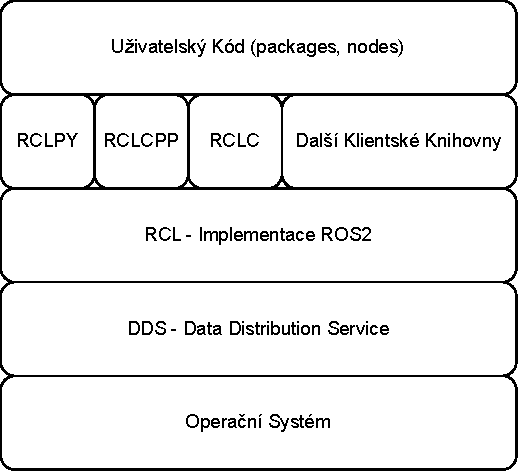
\includegraphics[scale=0.75]{obrazky-figures/ros_layers.pdf}
	\caption{Vrstvy ROS2}
	\label{fig:ros_layers}
\end{figure}

\subsection*{Vývoj v ROS2}
Nejvyšší organizační jednotkou v ROS2 je pracovní plocha(workspace). Jedná se o složku, která slouží k organizaci zdrojových souborů, jejich instalaci a následné spouštění. ROS2 jako takový se také kvalifikuje jako pracovní plocha a před použitím musí být nejprve aktivován. K tomu v Linuxu slouží příkaz \verb|source|. Aktivace pracovních ploch je akumulativní. To znamená, že v jeden moment jich může být aktivních hned několik najednou. Typicky se první aktivuje základní ROS2 instalace, která tvoří takzvanou underlay vrstvu. Vývojová pracovní plocha aktivována jako druhá, se pak nazývá overlay. Pokud má overlay nějaké závislosti, měly by být uspokojeny v underlay.
Zdrojové soubory v rámci pracovní plochy jsou organizovány do balíků (packages). Balík může obsahovat zdrojové soubory, knihovny a definice zpráv. Balíky na sobě můžou navzájem záviset (například balík, který využívá konkrétní rozhraní, závisí na jiném, který toto rozhraní definuje). \cite[str:~10-11]{ros2_introduction} 

\newpage
\noindent Následující strom zobrazuje typickou strukturu pracovní plochy a balíku:
\begin{center}
	\begin{forest}
		for tree={
			font=\ttfamily,
			grow'=0,
			child anchor=west,
			parent anchor=south,
			anchor=west,
			calign=first,
			inner xsep=7pt,
			edge path={
				\noexpand\path [draw, \forestoption{edge}] (!u.south west) +(7.5pt,0) |- (.child anchor) \forestoption{edge label};
			},
			before typesetting nodes={
				if n=1
				{insert before={[,phantom]}}
				{}
			},
			fit=band,
			before computing xy={l=15pt},
		}
		[Workspace
		[build / install /log {\hspace{3em}\# složky generované při kompilaci}
		]
		[launch {\hspace{2.5em}\# globální spouštěcí soubory}
		]
		[src {\hspace{4em}\# balíky}
		[package\_name {\hspace{2em}\#příklad jak vypadá python package}
		[package\_name {\hspace{2em}\#zdrojové python soubory}
		]
		[config {\hspace{2.5em}\# konfigurační soubory}
		]
		[launch {\hspace{2.5em}\# spouštěcí soubory pro uzly balíku}
		]
		[resource
		]
		[test
		]
		[package.xml {\hspace{1em}\#metadata o package}]
		[setup.cfg]
		[setup.py {\hspace{2.5em}\#instrukce pro kompilátor jak nainstalovat package}]
		]
		]
		]
	\end{forest}
\end{center}

\subsubsection*{Node}
Celý ROS2 systém je složený z uzlů (node), které mezi sebou navzájem komunikují. Každý uzel je vlastní výpočetní jednotka, která by měla plnit jeden specifický úkol. Tento přístup je podobný objektově orientovanému návrhu. Implementačně je uzel objekt, který dědí ze třídy \verb|Node|. \cite{ros2_documentation}
Uzly v ROS2 většinou nepotřebují běžet permanentně, ale pouze v~momentě, kdy nastane nějaká událost, kterou je potřeba obsloužit. Z toho důvodu existuje v ROS2 metoda \verb|spin()|, která uspí vykonávání uzlu, dokud jej není potřeba opět využít. Aby ROS2 šetřil výpočetní prostředky, využívá dva přístupy k určení, kdy bude potřeba uzel vzbudit. Prvním je iterative execution. Ten se používá u uzlů, které vykonávají svou činnost pravidelně, na nějaké předem dané frekvenci. Příkladem může být uzel pro obsluhu senzoru. Ten se v pravidelných intervalech zaktivuje, získá nová data, nějakým způsobem je zpracuje a~následně odešle dalším uzlům, které je potřebují pro svou činnost.
Druhým přístupem je event oriented execution. Zde je vyvolání řídícího cyklu důsledkem nějaké události. Typickou událostí je příchod zprávy od ostatních uzlů. Frekvenci spouštění těchto uzlů pak lze odvodit od frekvence příchozích zpráv. Příkladem může být uzel přijímající snímky z kamery, na kterých provede výpočet a vrátí odpověď. Frekvence spuštění je dána příchozími snímky, pokud přestanou přicházet, uzel bude neaktivní. \cite[str:~6]{ros2_introduction}

\begin{algorithm}[h!]
	\label{}
	\caption{\textsc{Definice a použití uzlu}}
	
	\DontPrintSemicolon
	\SetAlgoNoLine
	\SetAlgoNlRelativeSize{-1}
	\SetNlSty{}{}{:}
	\SetNlSkip{-1.1em}
	
	\BlankLine \Indp\Indpp
	
	\texttt{class CustomNode(Node):}\;
	\Indp\Indp
	\texttt{def \_\_init\_\_(self):}\;
	\Indp\Indp
	\texttt{super().\_\_init\_\_('node\_name')}\;
	\Indm\Indm\Indm\Indm
	
	\BlankLine
	
	\texttt{def main(args):}\;
	\Indp\Indp
	\texttt{rclpy.init(args=args)}\;
	\texttt{node = CustomNode()}\;
	\texttt{rclpy.spin(node)}\;
	\texttt{node.destroy\_node()}\;
	\texttt{rclpy.shutdown()}\;
\end{algorithm}

\newpage
\subsubsection*{Interface}
Jak už bylo řečeno, tak uzly ROS2 systému spolu komunikují posíláním zpráv. Aby si uzly navzájem rozuměly, musí mít tyto zprávy stejnou strukturu. K tomuto účelu slouží rozhraní~(interface). 

ROS2 obsahuje mnoho již vytvořených a vývojáři po celém světě používaných formátů. Tento přístup podporuje znovupoužitelnost vytvořeného kódu a šetří práci. Díky tomu může být software pro ovládání konkrétního kusu hardware implementován pouze jednou s~využitím standardního rozhraní a všichni ostatní jej pak mohou využít ve svých systémech. Pokud však standardní rozhraní nevyhovuje potřebám, lze si implementovat vlastní.\cite{ros2_documentation} Více o definici vlastních rozhraní na straně \pageref{theory:custom_interfaces}.

V kódu má každé rozhraní vygenerovanou vlastní třídu, která slouží k jeho reprezentaci. Instance této třídy jsou používány jako zprávy posílané mezi uzly. Data přenášená těmito zprávami se ukládají do atributů. Atributy těchto objektů mají strukturu danou originálním rozhraním.

\subsubsection*{Topic}
Je základním a také nejčastěji používaným způsobem, pomocí kterého spolu ROS2 uzly komunikují. Topic si lze představit jako analogii hardwarové sběrnice. Prakticky se jedná o~přesně pojmenované místo, do kterého může n uzlů publikovat data (Publish) a m odebírat co bylo posláno (Subscribe). Zprávy posílané do topicu mají přesný formát a jsou posílány asynchronně. Příkladem použití může být topic, do nějž posílá data uzel ovládající kameru a několik dalších uzlů, které tyto data potřebují, jej mohou číst. \cite[str:~6]{ros2_introduction}

\begin{algorithm}[h!]
	\label{}
	\caption{\textsc{Uzel odebírající zprávy z topicu}}
	
	\DontPrintSemicolon
	\SetAlgoNoLine
	\SetAlgoNlRelativeSize{-1}
	\SetNlSty{}{}{:}
	\SetNlSkip{-1.1em}
	
	\BlankLine \Indp\Indpp
	\texttt{self.create\_subscription(Interface, "topic\_name", self.callback\_function, qos\_profile)}\;
	
	\BlankLine
	\texttt{def callback\_function(self, msg: Interface):}\;
	\Indp\Indp
	\texttt{value = msg.item}\;
\end{algorithm}
Tento kód ukazuje, jak se může uzel přihlásit k odebírání zpráv z topicu. Nejprve je potřeba (typicky v konstruktoru třídy) zavolat zděděnou metodu. V tomto případě se jedná o \verb|create_subscription|, která vytvoří odběratelský objekt. Jako parametry potřebuje jméno, rozhraní, funkci pro zpětné volání (callback) a QoS profil. K invokaci funkce zpětného volání dochází vždy, když uzel příjme zprávu. Jako parametr je jí předán objekt reprezentující danou zprávu. \cite{ros2_documentation}

\begin{algorithm}[h!]
	\label{}
	\caption{\textsc{Jednoduchý uzel publikující data}}
	
	\DontPrintSemicolon
	\SetAlgoNoLine
	\SetAlgoNlRelativeSize{-1}
	\SetNlSty{}{}{:}
	\SetNlSkip{-1.1em}
	
	\BlankLine \Indp\Indpp
	\texttt{self.publisher = self.create\_publisher(Interface, "topic\_name", qos\_profile)}\;
	
	\BlankLine
	\texttt{output = Interface()}\;
	\texttt{output.item = some\_value}\;
	\texttt{self.publisher.publish(output)}\;
\end{algorithm}
Odesílání zpráv do topicu používá podobné principy jako jejich poslouchání. Jak bylo řečeno, zprávy jsou instance tříd reprezentující rozhraní. Proto je potřeba tuto instanci vytvořit, naplnit daty a následně předat metodě \verb|publish|. Ta je součástí předem vytvořeného \verb|publisher| objektu. \cite{ros2_documentation}

\subsubsection*{Service}
ROS2 služby (service) fungují na stejném principu jako klient--server komunikace známá z~počítačových sítí. Jedná se tedy o synchronní komunikaci, kde jeden uzel poskytuje nějakou službu a ostatní si na ni mohou poslat požadavek. Od serverového uzlu se předpokládá okamžitá odpověď, aby nedošlo k narušení řídícího cyklu volajícího uzlu. \cite[str:~6]{ros2_introduction}

\begin{algorithm}[h!]
	\label{}
	\caption{\textsc{Uzel poskytující službu}}
	
	\DontPrintSemicolon
	\SetAlgoNoLine
	\SetAlgoNlRelativeSize{-1}
	\SetNlSty{}{}{:}
	\SetNlSkip{-1.1em}
	
	\BlankLine \Indp\Indpp
	
	\texttt{self.srv = self.create\_service(Interface, "service\_name", self.callback\_function)}\;
	\BlankLine
	\texttt{def callback\_function(self, request, response):}\;
	\Indp\Indp
	\texttt{value = request.item}\;
	\texttt{response.item = some\_value}\;
	\texttt{return response}\;
	
\end{algorithm}
Tento kód demonstruje vytvoření služby. Hlavní změnou oproti předchozím příkladům jsou parametry funkce zpětného volání. Ty jsou nyní dva, požadavek (request) a odpověď (response). Principiálně se používají stejně jako u topiců. Jejich atributy tvoří strukturu přijaté / odesílané zprávy. Odpověď se tentokrát neodesílá metodou serveru, ale vrací se skrz návratovou hodnotu funkce. \cite{ros2_documentation}

\begin{algorithm}[h!]
	\label{}
	\caption{\textsc{Klientská strana služby}}
	
	\DontPrintSemicolon
	\SetAlgoNoLine
	\SetAlgoNlRelativeSize{-1}
	\SetNlSty{}{}{:}
	\SetNlSkip{-1.1em}
	
	\BlankLine \Indp\Indpp
	
	\texttt{self.client = self.create\_client(Interface, "service\_name")}\;
	\texttt{while not self.client.wait\_for\_service(timeout\_sec=1.0):}\;
	\Indp\Indp
	\texttt{pass}\;
	\Indm\Indm

	\BlankLine
	\texttt{def send\_request(self):}\;
	\Indp\Indp
	\texttt{self.req = Interface.Request()}\;
	\texttt{self.req.item = some\_value}\;
	\texttt{self.future = self.client.call\_async(self.req)}\;
	\texttt{rclpy.spin\_until\_future\_complete(self, self.future)}\;
	
	\BlankLine
	\texttt{response = self.future.result()}\;
	\texttt{value = response.item}\;
\end{algorithm}
\newpage
Klient potřebuje pro své fungování již existující službu. Tato podmínka vyplývá z faktu, že služby jsou určeny k úkolům, které lze vykonat relativně rychle a odpovědět na požadavek v krátkém čase. Klientská strana proto čeká synchronně. V případě že by servis neexistoval, klient by se zasekl v nekonečném čekání. Proto je hned v konstruktoru implementována kontrola, které nedovolí vytvoření uzlu, dokud není přítomen server. Čekání na odpověď od serveru je pak implementováno pomocí funkce \verb|spin_until_future_complete|. \cite{ros2_documentation}

\subsubsection*{Action} \label{theory:action}
Jedná se o rozšířenou verzi služeb. Akce z pravidla vykonává déle trvající požadavek. Například provedení řídícího manévru robota, který je prováděn v reálném světě a z pohledu uzlu se nejedná o krátkodobou záležitost. Akce, na rozdíl od služby, dokáže v průběhu vykonávání své činnosti odesílat průběžné aktualizace o aktuálním stavu zpět volajícímu uzlu. \cite[str:~6]{ros2_introduction} Implementačně akce funguje jako dvě služby a jeden topic. Cílová (goal) služba slouží k zaslání požadavku na server a jeho potvrzení. Výsledková (result) pak vrací výsledek operace. V průběhu vykonávání je zasílána zpětná vazba do topicu. \cite{ros2_documentation}

\begin{algorithm}[h!]
	\label{}
	\caption{\textsc{Implementace akčního serveru}}
	
	\DontPrintSemicolon
	\SetAlgoNoLine
	\SetAlgoNlRelativeSize{-1}
	\SetNlSty{}{}{:}
	\SetNlSkip{-1.1em}
	
	\BlankLine \Indp\Indpp
	
	\texttt{self.action\_server = ActionServer(self, Interface, "action\_name", self.execute\_callback)}\;
	
	\BlankLine
	\texttt{def execute\_callback(self, goal\_handle):}\;
	\Indp\Indp
	\texttt{goal\_handle.request.item}\;
	
	\BlankLine
	\tcp{odeslání zpětné vazby volajícímu}
	\texttt{feedback = Interface.Feedback()}\;
	\texttt{feedback.item = some\_value}\;
	\texttt{goal\_handle.publish\_feedback(feedback)}\;
	
	\BlankLine
	\tcp{úspěšné ukončení požadavku}
	\texttt{goal\_handle.succeed()}\;
	\texttt{result = Interface.Result()}\;
	\texttt{result.item = some\_value}\;
	\texttt{return result}\;
\end{algorithm}
Implementace akčního serveru kombinuje postupy představené u služeb a topiců dohromady. Jedinou novinkou je parametr \verb|goal_handle|. Ten slouží k interakci s vnitřní implementací akcí. Obsahuje v sobě přijatý požadavek, odesílatele (publisher) zpětné vazby a~také ovládání samotného akčního serveru. \cite{ros2_documentation}

\begin{algorithm}[h!]
	\label{}
	\caption{\textsc{Akční klient - zaslání požadavku}}
	
	\DontPrintSemicolon
	\SetAlgoNoLine
	\SetAlgoNlRelativeSize{-1}
	\SetNlSty{}{}{:}
	\SetNlSkip{-1.1em}
	
	\BlankLine \Indp\Indpp
	
 	\texttt{self.action\_client = ActionClient(self, Interface, "action\_name")}\;
 	
 	\BlankLine
 	\texttt{def send\_goal(self):}\;
 	\Indp\Indp
 	\texttt{goal\_msg = Servo.Goal()}\;
 	\texttt{goal\_msg.item = some\_value}\;
 	\texttt{self.action\_client.wait\_for\_server()}\;
 	\texttt{self.goal\_future = self.action\_client.send\_goal\_async(goal\_msg, self.feedback\_callback\_function)}\;
 	\texttt{self.goal\_future.add\_done\_callback(self.response\_callback\_function)}\;
	\Indm\Indm
    
\end{algorithm}
V porovnání s klientem služeb je ten akční výrazně složitější. Tento klient interaguje se serverem, který z pohledu uzlů vykonává velmi dlouhé úkoly. Komunikace je proto asynchronní a používá několik funkcí zpětného volání. \cite{ros2_documentation} Prvním krokem je odeslání požadavku. Hlavním rozdílem oproti službám je použití funkcí zpětného volání k přijmu odpovědi a případné zpětné vazby od serveru.

\begin{algorithm}[h!]
	\label{}
	\caption{\textsc{Akční klient - reakce na přijmutí nebo zamítnutí požadavku}}
	
	\DontPrintSemicolon
	\SetAlgoNoLine
	\SetAlgoNlRelativeSize{-1}
	\SetNlSty{}{}{:}
	\SetNlSkip{-1.1em}
	
	\BlankLine \Indp\Indpp
	
	\texttt{def response\_callback\_function(self, future):}\;
	\Indp\Indp
	\texttt{goal\_handle = future.result()}\;
	\texttt{if not goal\_handle.accepted:}\;
	\Indp\Indp
	\texttt{return}\;
	\Indm\Indm
	
	\BlankLine
	\texttt{self.result\_future = goal\_handle.get\_result\_async()}\;
	\texttt{self.result\_future.add\_done\_callback(self.result\_callback\_function)}\;
	\Indm\Indm
	
\end{algorithm}
Zpracování odpovědi bývá vždy téměř totožné. Cílem je zjistit, zda byl požadavek přijat. Pokud ano, tak následuje odeslání dotazu na výsledek operace, který je opět získán přes funkci zpětného volání. \cite{ros2_documentation}

\begin{algorithm}[h!]
	\label{}
	\caption{\textsc{Akční klient - funkce zpětného volání}}
	
	\DontPrintSemicolon
	\SetAlgoNoLine
	\SetAlgoNlRelativeSize{-1}
	\SetNlSty{}{}{:}
	\SetNlSkip{-1.1em}
	
	\BlankLine \Indp\Indpp
	
	\BlankLine
	\texttt{def feedback\_callback\_function(self, msg):}\;
	\Indp\Indp
	\texttt{feedback = msg.feedback}\;
	\texttt{value = feedback.item}\;
	\Indm\Indm
	
	\BlankLine
	\texttt{def result\_callback\_function(self, future):}\;
	\Indp\Indp
	\texttt{result = future.result().result}\;
	\texttt{value = result.item}\;

\end{algorithm}
Tyto bloky už pouze ukazují, jak vypadají jednoduché funkce pro zpracování zpětné vazby a získání výsledku operace.

\subsubsection*{Definice vlastních rozhraní} \label{theory:custom_interfaces}
Jak už bylo řečeno, ROS2 disponuje standardními rozhraními. Existují ale případy, kdy tyto rozhraní nevyhovují a je potřeba si vytvořit vlastní. Každý druh komunikace mezi uzly má svou vlastní příponu pro definování rozhraní. \cite{ros2_introduction}

Prvním jsou \verb|.msg| zprávy. Tento formát je využíván topicy. Jedná se o seznam, kde je každá položka definována jako dvojice datový typ a název (případně komentář).
\begin{verbatim}
	int32 angle #comment
	string direction
\end{verbatim}

Druhým je \verb|.srv|. Slouží pro definici struktury požadavků a odpovědí zasílaných mezi službou a jejími klienty. Tento soubor obsahuje dvě části, požadavek a odpověď, každá je tvořena seznamem položek a jsou odděleny řádkem \verb|---|. 
\begin{verbatim}
	int32 a
	int32 b
	---
	int64 sum
\end{verbatim}

Poslední je \verb|.action| soubor. Slouží pro komunikaci mezi akčním serverem a klientem. Definice se skládá ze tří seznamů, jeden pro požadavek, druhý pro odpověď a poslední pro zpětnou vazbu.
\begin{verbatim}
	float32 goal_angle
	---
	bool response
	---
	float32 current_angle
\end{verbatim}

\subsubsection*{Parametry}
ROS2 uzly mohou definovat parametry. V jednodušších případech fungují stejně jako argumenty funkcí. Umožňují předat dynamické hodnoty při spuštění uzlu. Příkladem může být uzel, sloužící k obsluze periferního zařízení. Parametrem mu jsou předány čísla GPIO pinů, na které je dané zařízení připojeno. Parametry ROS2 uzlů jsou však pokročilejší. Každý uzel zdědí z \verb|Node| třídy několik služeb. Ty lze volat za běhu uzlu a umožňují jednak získat aktuální hodnoty parametrů, ale také je změnit. Následující kód demonstruje deklaraci a~použití parametrů uvnitř uzlu. \cite[str:~37-39]{ros2_introduction}

\begin{algorithm}[h!]
	\label{}
	\caption{\textsc{Použití parametrů v kódu}}
	
	\DontPrintSemicolon
	\SetAlgoNoLine
	\SetAlgoNlRelativeSize{-1}
	\SetNlSty{}{}{:}
	\SetNlSkip{-1.1em}
	
	\BlankLine \Indp\Indpp
	
	\tcp{deklarace parametru, typicky v konstruktoru}
    \texttt{self.declare\_parameter('parameter\_name', 'default\_parameter\_value')}\;
	
	\BlankLine
	\tcp{získání hodnoty parametru}
	\texttt{param = self.get\_parameter('parameter\_name').get\_parameter\_value().string\_value}\;
	
	\BlankLine
	\tcp{nastavení hodnoty parametru}
	\texttt{new\_param = rclpy.parameter.Parameter('parameter\_name',}\;
	\Indp\Indp
	\texttt{rclpy.Parameter.Type.STRING,}\;
	\texttt{'default\_parameter\_value'}\;
	\Indm\Indm
	\texttt{)}\;
	\texttt{new\_param\_list = [new\_param]}\;
	\texttt{self.set\_parameters(new\_param\_list)}\;

\end{algorithm}

\newpage
\subsubsection*{Konfigurační soubory}
Konfigurační soubory v ROS2 slouží k usnadnění práce s parametry. Výhody, které konfigurační soubory přinášejí, jsou následující. Oddělují hodnoty parametrů od spouštěcích souborů. Umožňují provádět změny konfigurace na jednom místě. A uzly, které jich používají velké množství, lze jednodušeji spouštět. Konfigurační soubory používané v ROS2 umožňují jedním souborem předávat parametry více uzlům. Obsah takového souboru vymezuje části specifické pro konkrétní uzly, ale také generické parametry aplikovatelné na všechny. Konfigurační soubory se typicky umisťují do složky \verb|config| v kořenovém adresáři balíku a používají formát \verb|.yaml|. Následující kód demonstruje jejich strukturu. \cite{ros2_documentation}

\begin{algorithm}[h!]
	\label{}
	\caption{\textsc{Struktura konfiguračního souboru}}
	
	\DontPrintSemicolon
	\SetAlgoNoLine
	\SetAlgoNlRelativeSize{-1}
	\SetNlSty{}{}{:}
	\SetNlSkip{-1.1em}
	
	\BlankLine \Indp\Indpp
	
	\tcp{parametry pro konkrétní uzel}
	\texttt{node\_name:}\;
	\Indp
	\texttt{ros\_\_parameters:}\;
	\Indp
	\texttt{int\_param: 16}\;
	\texttt{double\_param: 3.14 \#comment}\;
	\texttt{string\_param: "radians"}\;
	
	
	\BlankLine \Indm\Indm
	\tcp{wildcard, parametry pro všechny uzly}
	\texttt{/**: \dots}\;
	
\end{algorithm}

\subsubsection*{Launch file}
ROS2 systém se skládá z velkého množství navzájem komunikujících uzlů. Spouštění každého uzlu zvlášť by bylo pracné a zdlouhavé. Proto existují spouštěcí (launch) soubory, které mají za úkol nastartovat ROS2 systém. Možnými formáty pro psaní těchto souborů jsou \verb|Python|, \verb|yaml| a \verb|xml|. V této práci jsou použité \verb|Python| spouštěcí soubory. Základní struktura těchto souborů je vždy stejná. Funkce, kterou musí každý definovat se jmenuje \verb|generate_launch_description|. Návratovou hodnotou je objekt \verb|LaunchDescription| jehož obsahem jsou jednotlivé cíle, které mají být vykonány. Následující kód obsahuje příklad jednoduchého spouštěcího souboru se dvěma cíli. Jedním z nich je klasické spuštění uzlu. Je mu předán parametr a jeden z jeho topiců je přemapován na jiné jméno. Přemapování je užitečná funkcionalita, která pomáhá s kompatibilitou uzlů. Druhý cíl pak volá jiný spouštěcí soubor. Běžně se spouštěcí soubory používají minimálně na dvou úrovních. Vyšší se nacházejí na úrovni pracovní plochy. Jejich cílem je spuštění větší části ROS2 systému. Používají k tomu volání nižších spouštěcích souborů. Ty se nacházejí na úrovni balíků. Mají za úkol spustit a nakonfigurovat konkrétní uzel. \cite[str:~35-37]{ros2_introduction}

\begin{algorithm}[h!]
	\label{}
	\caption{\textsc{Launch file}}
	
	\DontPrintSemicolon
	\SetAlgoNoLine
	\SetAlgoNlRelativeSize{-1}
	\SetNlSty{}{}{:}
	\SetNlSkip{-1.1em}
	
	\BlankLine \Indp\Indpp
	
	\texttt{def generate\_launch\_description():}\;
	\Indp\Indp
	
	\tcp{spuštění konkrétního uzlu}
	\texttt{goal = Node(}\;
	\Indp\Indp
	\texttt{package='package\_name',}\;
	\texttt{executable='node\_name',}\;
	\texttt{namespace='namespace\_name',}\;
	\texttt{parameters=[\{}\;
	\Indp\Indp
	\texttt{'param\_name' : param\_value,}\;
	\Indm\Indm
	\texttt{\}],}\;
	\texttt{remappings=[}\;
	\Indp\Indp
	\texttt{('topic\_name', 'different\_topic\_name'),}\;
	\Indm\Indm		
	\texttt{]}\;
	\Indm\Indm	
	\texttt{)}\;
	
	\tcp{zavolání dalšího launch souboru}
	\texttt{other\_goal = IncludeLaunchDescription(}\;
	\Indp\Indp
	\texttt{PythonLaunchDescriptionSource([}\;
	\Indp\Indp
	\texttt{PathJoinSubstitution([}\;
	\Indp\Indp
	\texttt{FindPackageShare('package\_name'), 'launch', 'node\_name.py'}\;
	\Indm\Indm
	\texttt{])}\;
	\Indm\Indm	
	\texttt{]),}\;
	\Indm\Indm
	\texttt{)}\;
		
	\texttt{return LaunchDescription([}\;
	\Indp\Indp
	\texttt{goal,}\;
	\texttt{other\_goal}\;
	\Indm\Indm
	\texttt{])}\;
		
\end{algorithm}

\subsection*{Nástroje příkazové řádky}
Jak už bylo řečeno, tak ROS2 systémy se skládají z velkého množství navzájem komunikujících uzlů. Taková struktura je vhodná na organizaci a modularitu. Naopak pro ladění chyb v rozsáhlejším systému by mohla být problematická. ROS2 proto disponuje sadou nástrojů, které mají za úkol pomoci vývojářům zjišťovat informace o právě běžících uzlech. Obecný formát volání je:
\begin{verbatim}
	ros2 [command] [sub_command]
\end{verbatim}

Názvy příkazů jsou odvozené od jednotlivých ROS2 konceptů. Například \verb|node|, \verb|topic|, \verb|service| a \verb|param|. Podpříkazy pak reprezentují akce, které budou nad daným konceptem provedeny. Typicky se jedná o \verb|list| a \verb|info|, případně další, specifické pro konkrétní příkaz. Díky této struktuře a dobrému pojmenování jsou velice intuitivní a příjemné na používání. Zde je několik ukázkových a často používaných příkazů. \cite{ros2_documentation}

\begin{verbatim}
	#prints all active topics
	ros2 topic list 
	
	#subsribes to specific topic and prints out received messages
	ros2 topic echo /topic_name
	
	#prints structure of specified interface
	ros2 interface show /path_to_interface
	
	#prints node and all of its publishers, subscribers, services, actions
	ros2 node info /node_name
\end{verbatim}

\subsection*{Geometric transformation subsystem} \label{theory:tf}
Jedná se o podsystém ROS2, který realizuje geometrické transformace mezi jednotlivými částmi robota.
Vztah mezi dvěma objekty lze definovat pomocí posunu (translation) a~otočení (rotation). Matematicky jsou tyto složky reprezentovány maticemi, které po spojení vytváří výslednou transformační matici. Roboti se většinou skládají z velkého množství částí. Ty na sebe bývají navzájem zavěšeny a zároveň se jejich relativní pozice neustále mění. Není proto vhodné počítat tyto vztahy manuálně. A přesně z toho důvodu existuje TF. \cite[str:~63-67]{ros2_introduction}

\begin{equation}
	\begin{pmatrix}
		x_B\\
		y_B\\
		z_B\\
		1\\
	\end{pmatrix}
	=
	\begin{pmatrix}
		R_{A\rightarrow B}^{xx} & R_{A\rightarrow B}^{xy} & R_{A\rightarrow B}^{xz} & T_{A\rightarrow B}^x\\
		R_{A\rightarrow B}^{yx} & R_{A\rightarrow B}^{yy} & R_{A\rightarrow B}^{yz} & T_{A\rightarrow B}^y\\
		R_{A\rightarrow B}^{zx} & R_{A\rightarrow B}^{zy} & R_{A\rightarrow B}^{zz} & T_{A\rightarrow B}^z\\
		0 & 0 & 0 & 1\\
	\end{pmatrix}
	*
	\begin{pmatrix}
		x_A\\
		y_A\\
		z_A\\
		1\\
	\end{pmatrix}
\end{equation}

\begin{center}
	Matice pro manuální výpočet transformace
\end{center}

Základním prvkem, se kterým TF pracuje je takzvaný frame, neboli rám. Rám reprezentuje nějakou část robota, jako senzor, kolo a podobně. Tyto rámy jsou uspořádány do stromové struktury, kde má každý uzel vždy jednoho předka. Podle konvence je kořenovým rámem robota \verb|base_link|. Ten se fyzicky nachází v jeho středu. Dalším běžným rámem je \verb|odom|. Ten reprezentuje vztah mezi aktuální pozicí robota a počátkem souřadného systému.~\cite{ros_reps}

Pro předávání transformačních dat jsou využívány dva topicy.
\begin{itemize}
	\item {\verb|/tf| - dynamické transformace, komponenty připojené přes serva, motory}
	\item {\verb|/tf_static| - statické transformace, komponenty navzájem pevně spojené}
\end{itemize}
Pro interakci s transportním subsystémem se nepoužívají běžné odběratelské a publikující objekty, jako tomu je u topiců.
Pro zasílání nových dat do TF systému slouží \\ \verb|TransformBroadcaster|. Ten se používá vesměs stejně jako klasický \verb|publisher|.  \cite{ros2_documentation} 

\begin{algorithm}[h!]
	\label{}
	\caption{\textsc{Transform Broadcaster}}
	
	\DontPrintSemicolon
	\SetAlgoNoLine
	\SetAlgoNlRelativeSize{-1}
	\SetNlSty{}{}{:}
	\SetNlSkip{-1.1em}
	
	\BlankLine \Indp\Indpp
	
    \texttt{self.tf\_broadcaster = tf2\_ros.TransformBroadcaster(self)}\;
 
 	\BlankLine
	\texttt{transform = TransformStamped()}\;
	\texttt{transform.header.stamp = current\_time.to\_msg()}\;
	\texttt{transform.header.frame\_id = parent\_frame}\;
	\texttt{transform.child\_frame\_id = child\_frame}\;
	\texttt{transform.transform.translation.x = translation}\;
	\texttt{transform.transform.rotation.w = quaternion}\;
	\texttt{self.tf\_broadcaster.sendTransform(transform)}\;
	
\end{algorithm}

\newpage
Pro získání dat z tf systému pak slouží \verb|TransformListener|. Ten neprovádí jednoduché čtení zpráv posílaných v topicu, ale umožňuje dotazování se tf systému na konkrétní transformace. Dotaz se skládá ze specifikování dvou rámců, mezi kterými je transformace hledána. Tyto dva rámce nemusí být v tf stromu přímí potomci. Cesta od jednoho k druhému může vést přes několik uzlů, ale dokud jsou navzájem dosažitelné, tak tf vrátí výslednou transformaci. Druhou částí dotazu je čas. Pokud je cesta mezi rámy delší, může se i během několika milisekund výrazně změnit výsledná transformace. Použití aktuálního času tak není vhodné, a proto se používá konkrétní časová značka. Specifikování času také umožňuje získávat pozice z minulosti. \cite{ros2_documentation}

\begin{algorithm}[h!]
	\label{}
	\caption{\textsc{Transform Listener}}
	
	\DontPrintSemicolon
	\SetAlgoNoLine
	\SetAlgoNlRelativeSize{-1}
	\SetNlSty{}{}{:}
	\SetNlSkip{-1.1em}
	
	\BlankLine \Indp\Indpp
	
	\texttt{self.tf\_buffer = Buffer()}\;
	\texttt{self.tf\_listener = TransformListener(self.tf\_buffer, self)}\;

	\BlankLine
	\texttt{t = self.tf\_buffer.lookup\_transform(}\;
	\Indp\Indp
	\texttt{to\_frame\_rel,}\;
	\texttt{from\_frame\_rel,}\;
	\texttt{rclpy.time.Time()}\;
	\Indm\Indm
	\texttt{)}\;
	
\end{algorithm}

\section{Formáty pro popis robotů}
Popisy slouží k reprezentaci struktury, vzhledu a fyzikálních vlastností reálných robotů v prostředí ROS2. Jedním z nejčastějších použití je generování transformačního stromu zmíněného v minulé sekci.

\subsubsection*{Unified robotics description format}
Urdf je primární formát, který ROS2 používá k popisu robotů. Samotný kód je složený primárně z \verb|<link>| a \verb|<joint>| prvků. Link(článek) reprezentuje fyzické části robota jako jeho tělo či kola. Články jsou složené ze tří složek. Těmi jsou fyzikální \verb|inertial|, vizuální \verb|visual| a kolizní \verb|colision|. Vizuální a kolizní složky bývají většinou stejné. Oddělené definice umožňují použít u komplexních objektů jednodušší kolizní složku a šetřit tak výkon. Fyzická složka definuje hmotnost a matici setrvačnosti. Joint(kloub) tvoří nějaký vztah mezi články. Klouby můžou být fixní nebo různými způsoby pohyblivé. Klasickým použitím pohyblivosti je buď částečná nebo kontinuální rotace kolem jedné z os. Kromě toho je možné definovat také lineárně pohyblivé klouby. \cite{ros2_documentation} 

\subsubsection*{XML macro}
Xacro lze použít na jakékoli XML soubory, ale primárně se používá k generování urdf. Cílem tohoto formátu je zjednodušení urdf souborů, které se při popisu složitějších robotů stávají dlouhé, nepřehledné a náchylné na chyby. Xarco tedy přidává funkce sloužící k~eliminaci těchto nedostatků. 
První z nich je možnost definovat konstanty. V urdf se často opakují stejné hodnoty na několika místech. Typickým případem může být definice vizuální a~kolizní části \verb|<link>| elementů které bývají často totožné. \cite{ros2_documentation} 
\begin{verbatim}
	<xacro:property name="wheel_radius" value="0.035" />
\end{verbatim}
Na konstanty pak navazuje vkládání matematických výrazů, místo statických hodnot.
\begin{verbatim}
	<cylinder radius="${wheel_diameter/2}" length="0.1"/>
\end{verbatim}
Hlavní funkcionalitou tohoto formátu jsou však makra. Ty umožňují zaobalit blok kódu a~přiřadit mu identifikátor, pomocí kterého lze takové makro vkládat na další místa v~kódu. 
Makra mohou na vstupu přijímat také parametry. V těle makra lze tyto parametry vkládat a~v~kombinaci s matematickými výrazy vytvářet komplexní definice.
\begin{verbatim}
	<xacro:macro name="identificator" params="name mass:=default_value">
\end{verbatim}
Posledním rozšířením, které xacro oproti urdf přináší, je možnost rozdělení definice robota do více souborů.
\begin{verbatim}
	<xacro:include filename="components.xacro"/>
\end{verbatim} 

\section{Gazebo simulátor} \label{theory:gazebo}
Jedná se o robotický simulátor. Slouží k vývoji a testování softwaru bez závislosti na konkrétním fyzickém stroji. Simulátor samotný je nástroj. Pro jeho použití je potřeba vytvořit světy a modely robotů, které bude simulovat. Nativní formát který Gazebo k tomuto účelu používá je \verb|sdf|.

\subsection*{Definice světa}
Definice světů pro Gazebo simulátor se skládají ze dvou základních částí. Nejprve se zpravidla definují obecné vlastnosti simulace. Těmi jsou parametry prostředí, fyzikální charakteristiky světa a pluginy. Druhou částí je naplnění světa objekty. Gazebo povoluje několik přístupů pro vkládání modelů do simulace. Nejjednodušší cestou je vytvoření základních tvarů přímo v definici světa.
\begin{verbatim}
	<box>
	    <size>8 0.1 0.2</size>
	</box>
\end{verbatim}
Druhou možností je využití \verb|<mesh>| tagu pro vložení komplexnějších objektů. Umožňuje totiž vložit soubor obsahující model vytvořený například v Bleneru. Poslední možností je načtení objektu z oficiální fuel knihovny. Ta obsahuje mnoho uživateli vytvořených modelů, které lze jednoduše vložit do světa. \cite{gazebo_documentation}

\subsection*{Definice robota}
Tvorba modelů pro Gazebo simulátor je v základu podobná jako tvorbě urdf / xacro definic používaných v ROS2. Proto se následující řádky zaměří na rozšířující tagy specifické pro simulátor. Ty jsou primárně dva \verb|<senzor>| a \verb|<plugin>|. Senzory se vždy přiřazují k~nějakému existujícímu \verb|<link>| elementu. Tento článek pak reprezentuje fyzické vlastnosti a vzhled daného senzoru. Konkrétní typ a potažmo i funkcionalita se určuje nastavením argumentu \verb|type|. Gazebo disponuje řadou, většinou komplexnějších, senzorů jako lidar a~hloubková kamera. Parametry zvoleného typu lze upravit v těle tagu a jsou specifické pro jednotlivé typy senzorů. \cite{gazebo_documentation}

Pluginy pak slouží k rozšíření funkcionality simulátoru. Základní instalace Gazeba obsahuje mnoho užitečných pluginů. Příkladem může být \verb|DiffDrive| nebo \verb|JointController|. První zmíněný simuluje řízení robota s diferenciálním podvozkem. Druhý umožňuje simulovat chování podobné servu. \cite{gazebo_documentation}

\section{Mapování a navigace}
Problém mapování a navigace je komplexní problematika, jejichž kompletní porozumění výrazně přesahuje rozsah této práce. Nástroje jako \verb|slam_toolbox| a \verb|Navigation 2| umožňují provádět mapování a navigaci na téměř jakémkoli robotovi. Jejich velkou výhodou je taky fakt, že je lze používat i bez hloubkového porozumění této problematiky.

\subsection*{Simultaneous localization and mapping}
SLAM řeší problém tvorby mapy neznámého prostředí a současné lokalizace robota na této mapě. Vysokoúrovňový princip fungování SLAM zobrazuje následující algoritmus. První krok, observation, získává data ze senzorů a extrahuje z nich významné vlastnosti (features) okolí. Druhým krokem je data association. Jeho úkolem je asociovat získané vlastnosti okolí s významnými body (landmarks) mapy. Další tři kroky se použijí v případě, kdy algoritmus ztratí informaci o aktuální pozici robota. Využitím kombinace dat ze senzorů, odometrie a dalších algoritmů mají za úkol lokalizovat aktuální pozici robota. Poslední dvojice pak slouží k zpřesnění výsledné mapy. Při pohybu robota vznikají malé odchylky v odometrii i~mapě. Tyto odchylky se postupně sčítají a delší trasy tak můžou mít relativně velkou chybu. Loop closure má za úkol zaznamenat moment, kdy se robot vrátí do pozice, ve které již v~minulosti byl. S touto informací může následně upravit mapu tak, aby byla tato odchylka eliminována. \cite[str:~414-418]{slam}

\newpage
\begin{algorithm}[h!]
	\label{}
	\caption{\textsc{SLAM}}
	
	\DontPrintSemicolon
	\SetAlgoNoLine
	\SetAlgoNlRelativeSize{-1}
	\SetNlSty{}{}{:}
	\SetNlSkip{-1.1em}
	
	\BlankLine \Indp\Indpp
	
	\texttt{repeat:}\;
	\Indp\Indp
	\texttt{(1)Observation}\;	
	\texttt{(2)Data association}\;
	\texttt{\textbf{if} tracking failure detected \textbf{then}}\;
	\Indp\Indp
	\texttt{(3)Relocalitation}\;
	\texttt{(4)Motion estimation}\;
	\texttt{(5)Optimization}\;
	\Indm\Indm
	\texttt{\textbf{if} loop closure detected \textbf{then}}\;
	\Indp\Indp
	\texttt{(6)Loop closure correction}\;
	\texttt{(7)New landmark initialization}\;
	
\end{algorithm}
\begin{center}
	\vspace{-2em}
	Tento algoritmus pochází z \cite[str:~414]{slam}
\end{center}

\subsection*{Navigation 2} \label{theory:nav2}
Cílem knihovny Navigation 2 je pokročilé řízení robotů. Pomocí mapy a transformací zvládá navigovat roboty skrze rozsáhlá prostředí. K rozhodování tato knihovna používá Behaviorální stromy. Požadavky na navigaci jsou přijímány pomocí akcí. \cite{nav2_documentation}

V ROS2 systému je Nav2 tvořeno několika navzájem provázanými a spolupracujícími uzly. Dalo by se říct, že se jedná o svůj vlastní podsystém. Hlavními uzly, které Nav2 používá jsou \verb|Planner|, \verb|Controller|, \verb|Smoother| a \verb|Recovery|. Všechny tyto uzly jsou modulární. Jejich chování tak lze měnit použitím různých pluginů. Planner má za úkol vytvořit trajektorii pro navigaci. Úkolem Controlleru je řízení robota podél vypočítané trajektorie do cíle. Recovery pak řeší případy, kdy se robot od této trajektorie odchýlí. \cite{nav2_documentation}

\chapter{Implementace ROS2 systému}
Zaměřením této kapitoly je vytvořený ROS2 systém. Následující strany popisují principy použité k implementaci uzlů, ale také demonstrují praktické příklady použití ROS2 funkcionalit.

\section{Struktura systému}
Před popisem konkrétních uzlů a jejich rolí ve vytvořeném ROS2 systému bude vhodné nejprve přestavit jeho strukturu z abstraktnějšího pohledu.

Úkolem ROS2 systému je řízení robotické aplikace. Tento úkol lze velmi obecně rozdělit do dvou částí. Na hardwarově bližší úrovni je ovládání jednotlivých komponent robota. Jedná se o část tvořící jádro systému, bez kterého nelze implementovat vyšší, složitější úlohy. Těmi je řízení robota jakožto celku. Rozdělení vytvořeného systému do těchto bloků zobrazuje obrázek \ref{fig:system_structure}. 

\begin{figure}[h!]
	\centering
	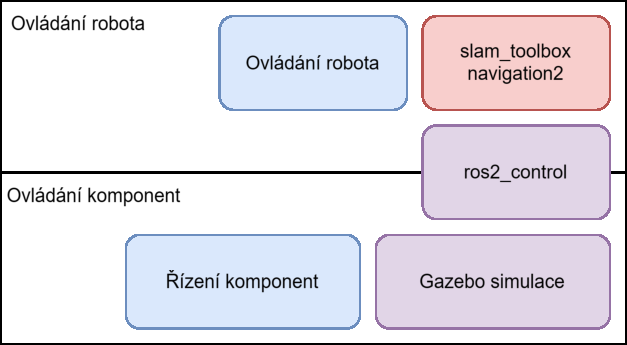
\includegraphics[scale=0.75]{obrazky-figures/system_structure.pdf}
	\caption{Abstraktní struktura výsledného systému}
	\label{fig:system_structure}
\end{figure}

Bloky strukturálních diagramů jsou také odlišeny barevně. Barva určuje, jak velká část dané oblasti byla implementována v rámci této práce. \textcolor[RGB]{108,142,191}{Modré} části jsou složeny z~ROS2 uzlů, které byly, s občasným využitím pomocných knihoven, zcela implementovány jako součást této práce.\footnote{výjimkou je uzel pro získávání dat z lidar senzoru, který byl jen s minimálními modifikacemi převzat} Pro \textcolor[RGB]{184,84,80}{červené} pak platí naprostý opak. Z většiny se jedná o funkcionalitu třetí strany. Hlavní prací v této části byla příprava existujícího ROS2 systému tak, aby těmto nástrojům poskytl všechny data, potřebné pro jejich fungování. Zároveň bylo také potřeba pochopit vnitřní strukturu těchto nástrojů a upravit jejich konfiguraci tak, aby lépe vyhovovala použitému robotu. Poslední, \textcolor[RGB]{150,115,166}{fialové}, části jsou někde na pomezí těchto extrémů. Gazebo simulátor společně s \verb|ros_gz_bridge| jsou existující nástroje. V rámci této práce byl vytvořen model pro reprezentaci robota Adeept AWR 4WD v simulátoru a několik ukázkových světů. Také byl upraven ROS2 systém, aby zajistil kompatibilitu řídících uzlů se simulovaným hardwarem. V souvislosti s ros2\_control byl implementován hardware plugin pro ovládání motorů. Ovladač diferenciálního pohybu byl využit z knihovny.

\begin{figure}[h!]
	\centering
	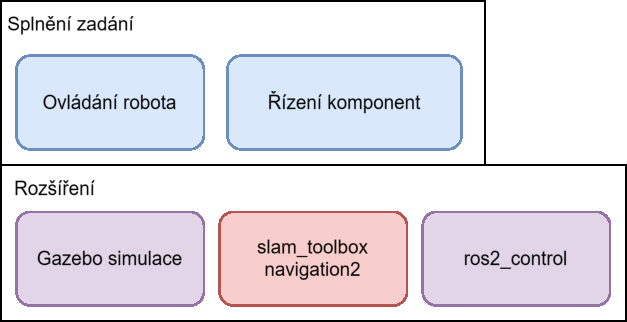
\includegraphics[scale=0.75]{obrazky-figures/zadání.pdf}
	\caption{Rozšířené části systému a zadání}
	\label{fig:zadani}
\end{figure}

\subsection*{Distribuovanost}
Řídící jednotky robotů bývají z pohledu výpočetního výkonu relativně slabá zařízení. Výpočetně náročné uzly mohou mít problémy s během na těchto zařízeních. Z toho a dalších důvodů umožňuje ROS2 distribuovat uzly mezi více fyzických zařízení. Z vývojářského pohledu je distribuovanost zcela v režii ROS2. Jediný předpoklad pro její fungování je vzájemná dosažitelnost zařízení přes počítačovou síť. Druhým požadavkem je nastavení stejného DOMAIN\_ID na obě zařízení, což je ve výchozím nastavení splněno. Ve správně fungujícím distribuovaném systému mohou uzly běžící na různých zařízeních navzájem komunikovat a interagovat stejně jako by běžely na jednom. V práci se tedy předpokládá, že systém bude rozdělen podle obrázku \ref{fig:distribuovanost}.

\begin{figure}[h!]
	\centering
	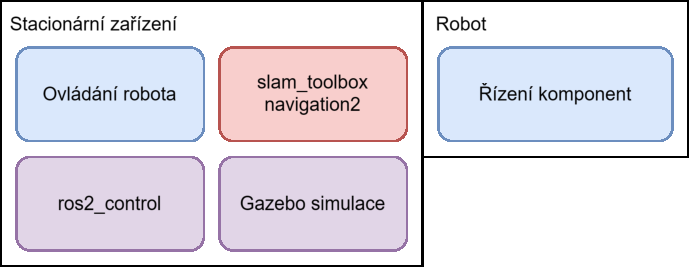
\includegraphics[scale=0.75]{obrazky-figures/distribuovanost.pdf}
	\caption{Distribuovanost vytvořeného systému}
	\label{fig:distribuovanost}
\end{figure}

\section{Uzly pro ovládání komponent}
Z pohledu vzdálenosti od hardwaru se jedná o nejnižší uzly. Úkolem těchto uzlů je využít rozhraní poskytnuté danou komponentou k jejímu ovládání a následnému zpřístupnění její funkcionality zbytku ROS2 systému.

\subsection*{Adeept kit}
Nejprve budou probrány uzly, sloužící k řízení komponent pocházejících z Adeept kitu. Každá následující podsekce reprezentuje jeden uzel, vytvořený v rámci této práce, sloužící k ovládání jedné z komponent.

\subsubsection*{Motory} \label{implementation:motors}
Jak už bylo řečeno v teoretické části, součástí Robot HAT je také full-bridge ovladač. Řídící uzel \verb|dc_motor_node| s tímto obvodem interaguje přímo pomocí GPIO pinů. K ovládání GPIO pinů byl použit Python modul \verb|RPi.GPIO|.\footnote{\url{https://pypi.org/project/RPi.GPIO/}} Zbytek řízení motorů už realizuje přímo uzel nastavováním hodnot vývodů \verb|In| a úpravou PWM frekvence na vývodu \verb|En|.

Od zbytku ROS2 systému uzel přijímá příkazy pomocí \verb|cmd_vel| (command velocity) topicu. Jedná se o běžně používané jméno pro zasílání příkazů na pohyb robota. Zprávy v tomto topicu jsou typu \verb|geometry_msgs/msg/Twist|. Robot s diferenciální nápravou se může pohybovat pouze v přímo vpřed / vzad, nebo otáčet do stran. Z Twist zprávy jsou pro něj tedy důležité pouze dvě složky \verb|linear.x| a \verb|angular.z|. Pomocí nich lze spočítat výsledná rychlost otáčení kol na jedné a druhé straně.

\begin{equation}
	\omega_L = \frac{V - \omega * b/2}{r}
\end{equation}
\begin{equation}
	\omega_R = \frac{V + \omega * b/2}{r}
\end{equation}

\noindent Kde $\omega_L$ a $\omega_R$ jsou výsledné rychlosti motorů v $[rad/s]$. $V$ je zadaná lineární a $\omega$ úhlová rychlost v $[m/s] a [rad/s]$. $b$ je rozpětí mezi koly a $r$ poloměr kola v $[m]$. \cite{diff_drive}

\begin{figure}[h!]
	\centering
	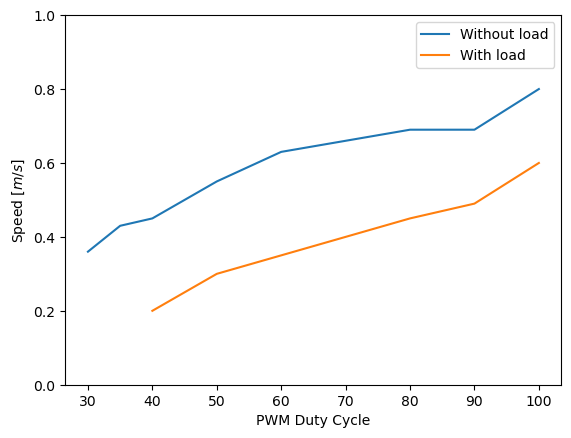
\includegraphics[scale=0.75]{obrazky-figures/motors_graph.png}
	\caption{Graf rychlosti robota pro různé hodnoty střídy motorů}
	\label{fig:motor_pwm_graph}
\end{figure}
Graf \ref{fig:motor_pwm_graph} zobrazuje lineární rychlost robota pro různé hodnoty PWM střídy motorů. Měření pod zátěží bylo zaznamenáno jako vzdálenost, kterou robot ujede za jednu vteřinu. Hodnoty bez zátěže byly získány pomocí změření času jedné otáčky hřídele motoru. Získaný čas byl následně přepočítán na vzdálenost. Je zde vidět, že hodnoty střídy menší než 30-40\% nedokážou překonat fyzikální jevy (setrvačnost, tření, \dots) aby motory vůbec roztočily. Zároveň růst není zcela lineární. Pro potřeby řízení motoru jsou hodnoty dostatečně blízko, aby je řídící uzel za lineární považoval.

Problém s motory, který se pořádně projevil až u jednoho z rozšíření je jízda po oblouku (současný pohyb vpřed a zatáčení). Nejsem si zcela jistý, co je příčinou tohoto jevu, ale hodnoty vypočítané využitím předchozího vzorce nevedou na předpokládaný oblouk. K~ujištění, že není chyba na mé straně, byl v pozdější fázi využit framework ros2\_control k~řízení motorů. Ten realizuje výpočet kinematiky vlastním vestavěným ovladačem a výsledek byl stejný. Zde je důležité zmínit, že robot se po oblouku pohybovat dokáže, pouze na to vyžaduje větší rozdíl mezi rychlostmi kol.

\subsubsection*{Servo}
Adeept AWD 4WD je vybaven pouze jedním servem. Slouží k ovládání úhlu natočení kamery. Konkrétní použitý model je Adeept AD002. Úhel serva se nastavuje pomocí PWM signálu. Jeho generování zajišťuje čip PCA9685, který je součástí Robot HAT. V softwaru je k~jeho řízení použita knihovna \verb|Adafruit_PCA9685|.\footnote{\url{https://github.com/adafruit/Adafruit_Python_PCA9685}} Řídící uzel serva se jmenuje \verb|servo_node| a z pohledu ROS2 systému se jedná o demonstraci jednoduchého akčního serveru. Server příjme požadavek a zkontroluje limity. 
Rozsah pohybu serva je větší než prostor pro kameru, řídící uzel proto omezuje maximální a minimální hodnoty natočení serva. Následně pomalu otáčí servem a v průběhu odesílá zpětnou vazbou s aktuálním úhlem serva.

\subsubsection*{Kamera} \label{implementation:camera}
Zachytávání snímků kamery je realizováno pomocí knihovny OpenCV.\footnote{\url{https://opencv.org/}} Aby bylo možno dosáhnout relativně krátké odezvy při přehrávání videa, není obraz zaznamenáván v nativním rozlišení a snímkovací frekvenci kamery, ale byly použity snížené hodnoty. V základní konfiguraci je použito rozlišení 960 na 540 pixelů a snímkovací frekvence 20 hz.
Pro přenos snímků v ROS2 systému je použita zpráva vestavěného typu \verb|CompressedImage|. Před odesláním jsou ještě data zakódována do \verb|jpeg| formátu pomocí funkce z \verb|OpenCV| knihovny.

\begin{center}
	\begin{tabular}{| l | c c c |}
		\hline
		Formát & Base64 & Image & CompressedImage \\ 
		\hline
		Velikost zprávy: & 0,24 MB & 1,56 MB & 0,17 MB  \\ 
		\hline 
	\end{tabular} \\ \vspace*{0.5em}
	Hodnoty v této tabulce pocházejí z utility \verb|ros2 topic bw|
\end{center}

Před finálním rozhodnutím o použití \verb|CompressedImage| formátu bylo experimentováno také se zprávami typu \verb|Image|. Tento typ obsahuje více rozšiřujících informací o přenášeném obrázku jako jeho rozměry, použité kódování a podobně. Na první pohled se tedy zdá jako vhodnější formát. Snímky kamery jsou ale přenášené mezi dvěma různými zařízeními pomocí wifi připojení. Tento objemově větší formát tak přináší příliš velké zpoždění, které překonává použitelné hranice pro streamování. Na počátku vývoje byl použit ještě třetí možný přístup. Ten však nevyužívá ROS2 funkcionality, a proto byl později změněn. Tímto přístupem je zakódování přenášených snímků do \verb|base64| formátu a následné přenesení jako jednoduchou \verb|string| zprávu. Base64 kódování se ukázalo jako zcela funkční možnost dosahující podobných výsledků zpoždění jako má \verb|CompressedImage|.
 
\subsubsection*{Ultrazvukový senzor} \label{implementation:ultrasonic}
Jedná o model hc-sr04. Ten dokáže měřit vzdálenost od 2 cm do 400 cm s přesností na 3mm. Získávání dat z ultrazvukového senzoru je relativně jednoduché a nevyžaduje tedy externí knihovnu. Interakce se senzorem je zajištěna pomocí GPIO pinů. K jejich ovládání je opět použit modul \verb|RPi.GPIO|. 

Uzel zahajuje komunikaci vysláním pulzu na trig vodiči. Reakcí senzoru je zahájení měření. Uzel následně čeká na odpověď. Ta přijde na echo pinu. Její začátek je signalizován tím, že senzor nastaví echo pin na hodnotu jedna. V ten moment si uzel uloží časovou značku. Poté počká, než se echo pin vrátí zpět do nuly. V ten moment získává druhou značku. Pomocí těchto dvou momentů lze vypočítat výslednou vzdálenost. Výpočet vzdálenosti je podrobněji popsán v teoretické části (str:~\pageref{theory:ultrasonic}).

Do ROS2 systému tento uzel odesílá kromě pravidelné informace o aktuální vzdálenosti také dvě další zprávy. Tou první je jednoduché varování o detekci překážky. Uzel varuje, pokud je naměřená vzdálenost menší než zadaná hranice. Toto varování však zaznamená pouze překážky přímo před robotem. Druhá zpráva tak doplňuje tu první. Snaží se detekovat překážky, které můžou stále vést ke kolizi, ale senzor je již nedetekuje. 

\begin{figure}[h!]
	\centering
	\begin{minipage}[c]{0.5\textwidth}
		\centering
		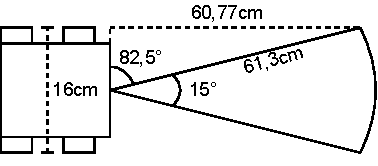
\includegraphics[scale=1.0]{obrazky-figures/ultrasonic_blind_spot.pdf}
	\end{minipage}%
	\begin{minipage}[c]{0.5\textwidth}
			$$\cos(82.5^\circ) = \frac{8\text{cm}}{\text{přepona}} \Rightarrow 61.3\text{cm}$$
			$$\sin(82.5^\circ) = \frac{\text{protilehlá}}{61.3\text{cm}} \Rightarrow 60.77\text{cm}$$
	\end{minipage}
	\caption{Překážky přehlédnutelné ultrazvukovým senzorem}
	\label{fig:ultrasonic_blind_spot}
\end{figure}

Obrázek \ref{fig:ultrasonic_blind_spot} demonstruje případy, které se snaží druhé varování zachytit. Je na něm vidět, že existuje meziprostor, ve kterém může překážka zmizet ze senzoru, ale i přes to vést ke kolizi s robotem. Tento meziprostor je na jedné straně ohraničen vzdáleností pro klasické detekování překážek, například 20 cm. Na druhé straně lze hranici vypočítat pomocí úhlu, ve kterém senzor detekuje překážky a šířky robota.
V tomto případě se jedná o přibližně 61 cm. Druhá zpráva tedy informuje o tom, že nějaká překážka zmizela z radaru v této potenciálně nebezpečné zóně.

\subsubsection*{Sledování čáry}
Posledním praktickým senzorem, kterým robot Adeept AWR disponuje je třícestný senzor na sledování čáry.
Komunikace je v tomto případě ještě jednodušší. Senzor má tři výstupy připojené na tři GPIO piny. Každá dvojice vysílače a senzoru má svůj vlastní vývod. Hodnoty těchto výstupů obsahují aktuální stav detekování čáry. Z pohledu uzlu tak stačí pravidelně číst stav těchto tří pinů a odesílat jej dále do ROS2 systému. K práci s GPIO piny tento uzel také používá modul \verb|RPi.GPIO|.

\subsubsection*{Led}
Součástí Adeept sady je také několik adresovatelných led diod. Jedná se o hardware, který je pro hlavní funkcionalitu naprosto nepotřebný. Ponechat však na robotu nevyužitý a neovládatelný hardware nedává smysl. Proto byl nakonec implementován uzel na jejich řízení. Z~pohledu ROS2 se jedná o klasickou službu. Požadavky obsahují RGB barevnou hodnotu, pro nastavení všech led zároveň. Řízení tohoto typu led pásku je komplexnější záležitost, a~proto je k jeho ovládání využit Python modul \verb|rpi_ws281x|.\footnote{\url{https://pypi.org/project/rpi-ws281x/}}
Aby tento modul mohl správně pracovat, vyžaduje spuštění s vyššími oprávněními. Důvodem k tomuto požadavku je fakt, že vnitřně využívá kód v jazyce C, který pracuje s GPIO piny přímo přes /dev/mem. Problém nastává v tom, že ROS2 při svém běhu nevyžaduje, a tedy ani nepoužívá zvýšená oprávnění. Z toho důvodu na tyto případy není připravený a prosté přidání \verb|sudo| před spouštěcí příkaz nefunguje. Toto lze obejít a spustit uzel s oprávněními podobnými příkazu \verb|sudo|. Avšak uzly spuštěné tímto způsobem nedokážou komunikovat s klasicky spuštěnými uzly. 
Problém je ve výsledku vyřešen použitím druhého skriptu. Ten obsahuje jen minimum kódu pro ovládání zmíněného modulu. V \verb|sudoers| je tomuto konkrétnímu souboru umožněno spuštění se \verb|sudo| oprávněními, aniž by bylo vyžadováno heslo. Tento skript je následně volán z hlavního uzlu použitím \verb|subprocess| modulu. Jedná se o velmi neelegantní řešení. Vzhledem k tomu, že se svícení LED diodami není důležitá funkcionalita a zbytečně upravuje systémově důležitý soubor \verb|sudoers|, je tento krok v instalačním skriptu volitelný.

\subsection*{Další hardware nad rámec Adeept kitu}
V tento moment byly probrány všechny uzly, které řídí komponenty stavebnice Adeept AWR 4WD. Následuje popis rozšíření původního hardwaru o další komponenty, které buď rozšiřují funkcionalitu robota, nebo usnadňují jeho použití.

\subsubsection*{Nabíjení}
V originální konfiguraci napájí robota dvě sériově zapojené 18650 baterie. V tomto zapojení poskytují napětí 8 V s maximálním proudem 4 A. Součástí Adeept Kitu jsou kolébky na baterie. Ty jsou přímo připojené k zátěži (robot HAT). Nabíjení baterií musí být realizováno externě. Tento způsob je nepohodlný, protože přístup ke kolébkám vyžaduje sundání kol robota. Prvním rozšířením je tedy přidání BMS a nabíjecí desky (obr:~\ref{fig:battery}). 
Nejrozšířenějším způsobem nabíjení baterií 18650 jsou desky s čipem TP4056. Jedná se o hojně dostupný produkt, který lze koupit v různých kombinacích ochran a vstupů pro napájení. Problémem je fakt, že tyto desky jsou určeny pro nabíjení jedné 18650 baterie. Potenciálním řešením pro paralelní zapojení je použití více těchto desek. Pro baterie zapojené sériově, které používá tento robot, jsou tyto desky nevhodné.
Lepší přístup je využití Battery Management System. Jak z názvu vyplývá, jedná se o desku pro správu baterií. BMS se vyrábí specificky pro konkrétní zapojení, které bude monitorovat. Použitý model je typu 2 S, pro dvě sériově zapojené baterie. Kromě kladného a záporného pólu disponuje také připojením pro bod mezi bateriemi. Tento bod umožňuje desce monitorovat stav každé z baterií zvlášť.
V~kombinaci s BMS je dále využita samotná nabíjecí deska. Jedná se o model, který na rozdíl od TP4056 nabíjí dvakrát vyšším nabíjecím napětím.

\begin{figure}[h!]
	\centering
	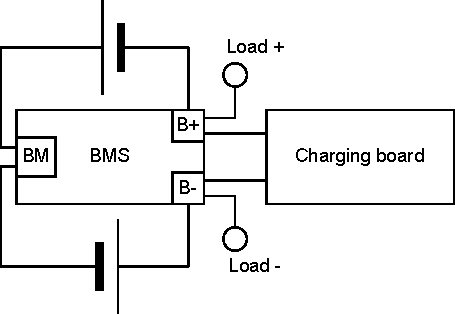
\includegraphics[scale=0.75]{obrazky-figures/battery_circuite.pdf}
	\caption{Zapojení BMS a nabíjecí desky}
	\label{fig:battery}
\end{figure}

\subsubsection*{Inertial mesurement unit - IMU}
Druhým rozšířením oproti originální stavebnici je přidání IMU senzoru. Konkrétně se jedná o model MPU5060. Ten disponuje tříosým akcelerometrem a gyroskopem. Uzel na jeho ovládání byl implementován v rámci této práce. Vnitřně využívá knihovnu třetí strany \verb|mpu6050-raspberrypi|.\footnote{\url{https://pypi.org/project/mpu6050-raspberrypi/}} Získaná data je nejprve potřeba vyčistit. Přímo v hardwaru je implementována dolní propusť, sloužící k eliminaci vibrací a jiných nechtěných vlivů. Nastavuje se zápisem do konfiguračního registru na adrese \verb|0x1A|, což lze provést využitím knihovní funkce \verb|set_filter_range|. Získaná data se nadále čistí softwarově. Protože se jedná o levný senzor, tak není zcela přesný a čtené hodnoty obsahují malé odchylky i~v~době, kdy by měly být nula. Proto se v softwaru aplikuje offset, který posune výsledky blíže k~reálným hodnotám. Dalším krokem může být získaná data průměrovat mezi více vzorky a~dosáhnout tak ještě většího utlumení výkyvů.

Do ROS2 systému tento uzel nejprve odesílá aktuální hodnoty zaznamenané senzorem, a~to pomocí zpráv typu Twist. Následně také posílá varování o kolizi, to detekuje v momentě, kdy \verb|cmd_vel| topic obsahuje příkaz pohybu, ale imu senzor čte výrazně odlišná data. Jako poslední tento uzel ještě odesílá odometrii. Odometrie udává transformaci aktuální pozice robota vůči počátku. Uzel tedy pravidelně čte hodnoty senzoru a integruje je, aby získal absolutní pozici robota. Největším problémem u získávání odometrie byl vliv gravitace na akcelerometr a fakt, že stejné zrychlení a zpomalení se ne vždy rovná. Gravitace vede na špatné hodnoty zrychlení v případě, že je robot nakloněn v nebo proti směru pohybu. Různé hodnoty akcelerace a decelerace je pravděpodobně způsobená rychlou změnou, kterou senzor nestihne vzorkovat dostatečně rychle.

\begin{figure}[h!]
	\centering
	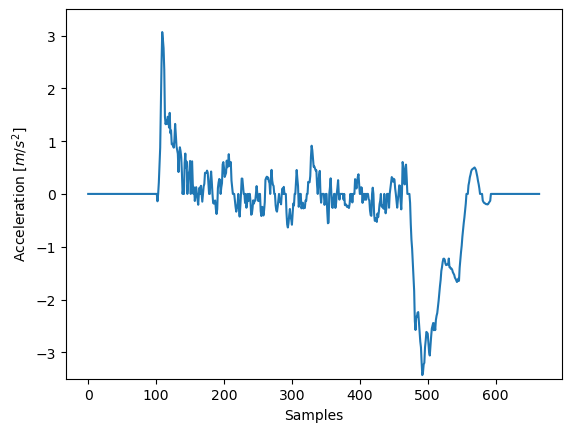
\includegraphics[scale=0.75]{obrazky-figures/accelerometer_graph.png}
	\caption[Graf výstupních hodnot akcelerometru]{Zobrazení hodnot akcelerometru v průběhu zrychlení a zastavení robota. Výsledná rychlost po zintegrování tohoto grafu je -0.1496m/s}
	\label{fig:accel_readings}
\end{figure}
Graf \ref{fig:accel_readings} zobrazuje případ, kdy došlo k špatnému zaznamenání zpomalení a výsledná rychlost je následně záporná. Důležité je zmínit, že případy, kdy dochází k špatnému měření, nejsou běžné (cca každé 15-20). Z grafu je také vidět, že když se robot pohybuje, je měření ovlivněno vibracemi motorů. Při testování se tento jev neprojevil dostatečně výrazně, aby ovlivnil funkcionalitu.

Ve finální verzi jsou tyto vlivy převážně eliminovány využitím dat z \verb|cmd_vel| topicu. Tento přistup umožňuje ignorovat výkyvy dat získaných z imu senzoru v momentech, kdy by podle příkazů z \verb|cmd_vel| měl být robot statický.

\subsubsection*{Light detection and ranging - Lidar}
Posledním a zároveň nejkomplexnějším přidaným senzorem je lidar. Konkrétním použitým modelem je LD 19 D 300. K jeho ovládání je využit již existující ROS2 balík \verb|ld19_lidar|.\footnote{\url{https://github.com/richardw347/ld19_lidar}} Výstupem tohoto uzlu jsou zprávy typu \verb|LaserScan| na topicu \verb|/scan|. Pro zajištění lepší kompatibility s \verb|slam_toolbox| byly v tomto uzlu provedeny menší změny v hlavičce odesílaných zpráv a byly odebrány nepotřebné výpisy, které zpomalovaly odesílání.

\subsubsection*{Přenos zvuku}
V zadání práce je zmíněno také téma teleprezence. Již probrané komponenty zajistí záznam videa a pohyb robota. K plnohodnotnější teleprezenci je však potřeba zajistit také přenos zvuku. Na rozdíl od videa by měl být ideálně obousměrný. Mozkem robota je mikropočítač Raspberry Pi 4, na kterém běží plnohodnotný operační systém. Připojení externích periferií jako mikrofon a reproduktory proto není problém. Řízení komponentů v tomto případě zajistí operační systém. ROS2 uzly se díky tomu můžou zaobírat pouze záznamem, přenosem a přehráváním dat. Pro tento účel byly vytvořeny dva uzly.

První slouží k nahrávání a odesílání audio dat. Pro záznam zvukového toku v reálném čase je použit Python modul \verb|sounddevice|.\footnote{\url{https://pypi.org/project/sounddevice/}} Tato knihovna, kromě jiného, disponuje také \verb|Stream| třídami. \verb|InputStream| umožňuje kontinuální záznam zvuku. Při inicializaci je jí (kromě dalších parametrů) předána funkce zpětného volání. K její invokaci dochází vždy, když je potřeba zpracovat nasnímaný blok dat. ROS2 nedisponuje standardním typem zprávy pro přenos zvukových dat. Je zde využit vlastní typ složený ze dvou polí o prvcích typu \verb|float32| (každé pro jeden kanál).

Druhý uzel pak realizuje příjem a přehrávání získaných dat. Jedná se o obrácenou verzi předchozího uzlu. Přijatá data jsou před přehráním uložena do bufferu. Důvodem je fakt, že přenos mezi dvěma uzly není zcela spolehlivý a datové bloky se mohou zpozdit. Pro přehrávání získaných dat je využita \verb|OutputStream| třída.

\begin{figure}[h!]
	\centering
	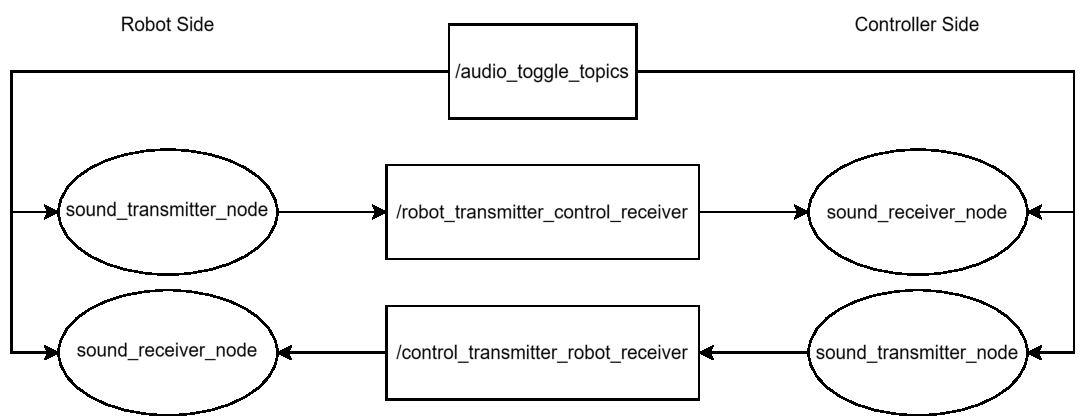
\includegraphics[scale=0.75]{obrazky-figures/audio_transfer_diagram.pdf}
	\caption{RQT Graf obousměrného přenášení zvuku}
	\label{fig:rqt_sound}
\end{figure}

Pro obousměrný přenos dat mezi robotem a stacionárním zařízením jsou použity dvě dvojice těchto uzlů (obr:~\ref{fig:rqt_sound}). Oba uzly disponují mechanismem pro pozastavení záznamu / přehrávání. 

\section{Řízení robota na vyšší úrovni}
V tento moment jsou připraveny všechny uzly pro ovládání komponent. Následuje sekce se zabývá řídícími uzly. Ty se nachází v balíku \verb|controllers| a byly implementovány v~rámci této práce. Jejich úkolem je zpracovávat data z několika hardwarových uzlů současně a~podle získaných dat řídit robota jako celek.

\subsection*{Manuální řízení}
Pro manuální řízení je systém vybaven dvěma uzly. První čte vstupy z klávesnice. Využívá k tomu modul \verb|pynput|.\footnote{\url{https://pypi.org/project/pynput/}} Druhý pak s pomocí \verb|pygame| knihovny získává vstupy ovladače.\footnote{\url{https://pypi.org/project/pygame/}} Oba uzly ovládají motory a servo pomocí jejich specifických rozhraní. Oba uzly také obsahují služby pro příjem příkazů sloužících k zastavení nebo spuštění smyček, které zajišťují zachytávání vstupu od uživatele (obr:~\ref{fig:rqt_manual}).

\begin{figure}[h!]
	\centering
	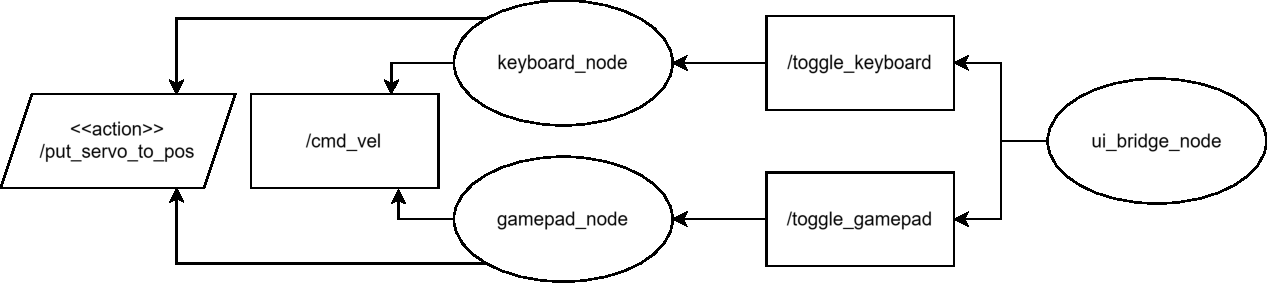
\includegraphics[scale=0.65]{obrazky-figures/manual_control_diagram.pdf}
	\caption{RQT Graf uzlů pro manuální řízení}
	\label{fig:rqt_manual}
\end{figure}

\subsection*{Pomocný uzel pro přesné otáčení robota}
Vzhledem k tomu, že použité motory nejsou opatřeny enkodéry, je, bez využití dalších senzorů, otáčení robota velice nepřesné. Motorům lze samozřejmě zadat konkrétní rychlost na určitý časový interval a dostat se tak na přibližně správnou orientaci. Z důvodu externích vlivů a nepřesností se opravdu jedná jen o přibližný úhel. Například setrvačnost hraje velkou roli při otáčení o úhly menší než 90° nebo při vyšším využití prostředků mikrokontroléru, můžou být reakce na příkazy zpožděné.
Proto byl vytvořen tento uzel, který využívá gyroskopická data z imu senzoru, aby zajistil, že se robot dokáže v případě potřeby otáčet o přesně dané úhly. V ROS2 systému se jedná o akční server. Přijímá požadavky a následně zasílá příkazy na \verb|cmd\_vel| topic. Podle hodnot získaných z imu pak postupně snižuje rychlost otáčení v závislosti na vzdálenosti od cílového úhlu (obr:~\ref{fig:alg_motor_controller}).

\begin{figure}[h!]
	\centering
	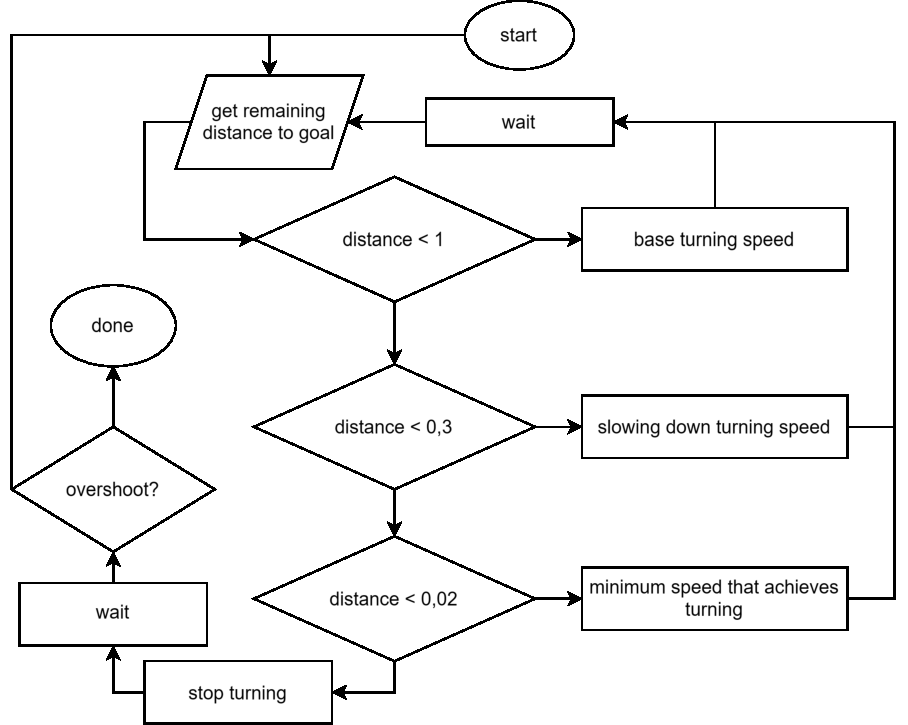
\includegraphics[scale=0.75]{obrazky-figures/precise_turning.pdf}
	\caption{Algoritmus přesného otáčení}
	\label{fig:alg_motor_controller}
\end{figure}

Z pohledu demonstrace ROS2 funkcionality tento uzel využívá pokročilejší možnosti akčního serveru. V případě standardního použití se pracuje pouze s \verb|execute_callback| funkcí (viz strana \pageref{theory:action}). V jejím těle by mělo proběhnou celé zpracování požadavku. Tento přístup však nelze použít vždy. Problém tohoto konkrétního uzlu je fakt, že v průběhu vykonávání požadavku jsou vyžadována data o aktuálním natočení robota. ROS2 uzly se točí (spin) a reagují při tom na události. V průběhu obsluh je točení pozastaveno. Z toho vyplývá, že v průběhu obsluhy požadavku akčního serveru nedochází k zpracování událostí a tedy ani získání nových dat z IMU senzoru. Akční server proto umožňuje definovat vlastní funkce zpětného volání pro jednotlivé události.

\begin{itemize}[leftmargin=*]
	\item{goal\_callback}
	\vspace*{-0.5em}
	\begin{itemize}
		\item{vyvolá se při příchodu požadavku, rozhoduje o jeho přijmutí nebo zamítnutí}
		\item{v případě tohoto uzlu: pokud již probíhá obsluha nějakého požadavku, tak jsou všechny nově příchozí zamítnuty, důvodem je fakt, že po dokončení aktuálního cíle bude výsledná orientace robota jiná, než když byly tyto požadavky zaslány, což s~největší pravděpodobností znamená, že již nejsou platné}
	\end{itemize}
	\item{handle\_accepted\_callback}
	\vspace*{-0.5em}
	\begin{itemize}
		\item{vyvolá se po přijmutí cíle}
		\item{v tomto uzlu zahajuje zpracování požadavku}
	\end{itemize}
	\item{execute\_callback}
	\vspace*{-0.5em}
	\begin{itemize}
		\item{měl by obsahovat hlavní funkcionalitu akčního serveru, rozhoduje o úspěchu požadavku}
		\item{v tomto uzlu je volán aby ukončil vykonávání požadavku (úspěšné i neúspěšné)}
	\end{itemize}
	\item{cancel\_callback}
	\vspace*{-0.5em}
	\begin{itemize}
		\item{vyvolán když klient zažádá o zrušení vykonávání cíle, rozhoduje o jeho přijmutí nebo zamítnutí}
	\end{itemize}
\end{itemize} 

Funkce zpětného volání mají přesně dané rozhraní, které musí následovat.
\begin{algorithm}[h!]
	\label{}
	\caption{\textsc{Příklad funkce zpětného volání akčního serveru}}
	
	\DontPrintSemicolon
	\SetAlgoNoLine
	\SetAlgoNlRelativeSize{-1}
	\SetNlSty{}{}{:}
	\SetNlSkip{-1.1em}
	
	\BlankLine \Indp\Indpp
	
	\texttt{def goal\_callback(self, goal\_request):}\;
	\Indp\Indp
	\texttt{if self.goal\_handle is not None and self.goal\_handle.is\_active:}\;
	\Indp\Indp
	\texttt{return GoalResponse.REJECT}\;
	\Indm\Indm
	\texttt{else:}\;
	\Indp\Indp
	\texttt{return GoalResponse.ACCEPT}\;

\end{algorithm}

\subsection*{Bloudění}
Náhodné bloudění robota po místnosti je základním autonomním pohybem. Cílem tohoto režimu je náhodný pohyb robota v prostoru, s cílem vyhýbat se překážkám.

K získávání informací o svém okolí používá tento uzel data ze dvou senzorů (obr:~\ref{fig:rqt_wandering}). Prvním je ultrazvukový senzor vzdálenosti. Ten je umístěn na přední straně robota a detekuje překážky v 15° úhlu před robotem. Druhým použitým senzorem je IMU. Přímo z něj získává pouze varování o kolizi. Nepřímo jej využívá při přesném otáčení s využitím uzlu \verb|motor_controller_node|.

\begin{figure}[h!]
	\centering
	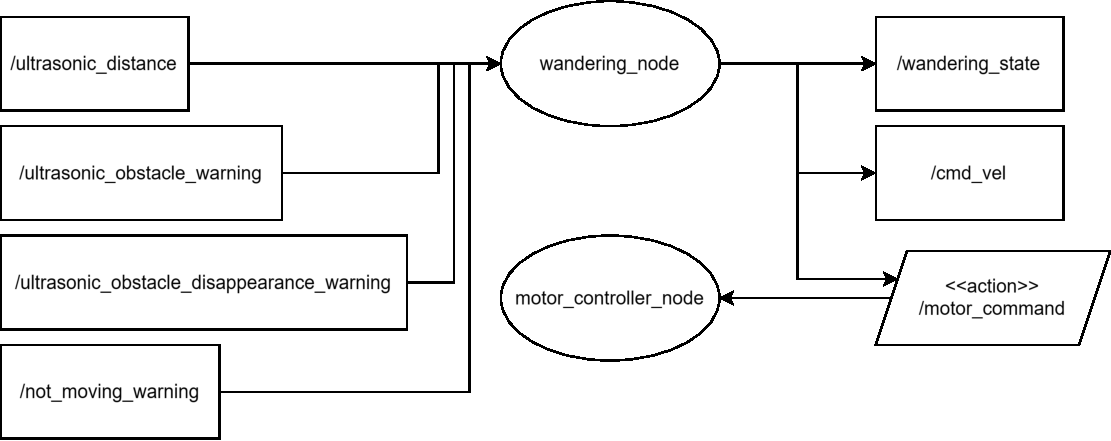
\includegraphics[scale=0.75]{obrazky-figures/wandering_rqt.pdf}
	\caption{RQT Graf bloudění}
	\label{fig:rqt_wandering}
\end{figure}

Jádrem implementace je konečný automat. Ten byl v průběhu vývoje obohacen o další funkcionalitu. Primárně bylo potřeba reagovat na externí události a volat funkce jiných uzlů. Výsledný kód tedy není čistým konečným automatem. Z abstraktnějšího pohledu má tento režim tří hlavní chování. Tím prvním je jednoduchý pohyb vpřed. Další dvě zajímavější pak realizují vyhýbání se překážkám. Úvodní stavy těchto chování jsou \verb|OBSTACLE| a~\verb|SCAN_START|.

\verb|OBSTACLE| má za úkol reagovat a vyřešit překážky nacházející se přímo před robotem. Detekování a přechod do tohoto stavu zajišťuje buď zpráva od ultrazvukového senzoru o~překážce nacházející se příliš blízko, nebo zpráva od imu senzoru varující o kolizi robota s~objektem.

Algoritmus hledání volné cesty je zobrazen na následujícím diagramu (obr:~\ref{fig:alg_obstacle}). Ve zkratce funguje následovně. V náhodném pořadí zkontroluje obě strany robota. Pokud na jedné z~nich najde volný prostor ihned tudy pokračuje v jízdě. Pokud je v obou směrech překážka, vrací se zpět odkud přijel.

\begin{figure}[h!]
	\centering
	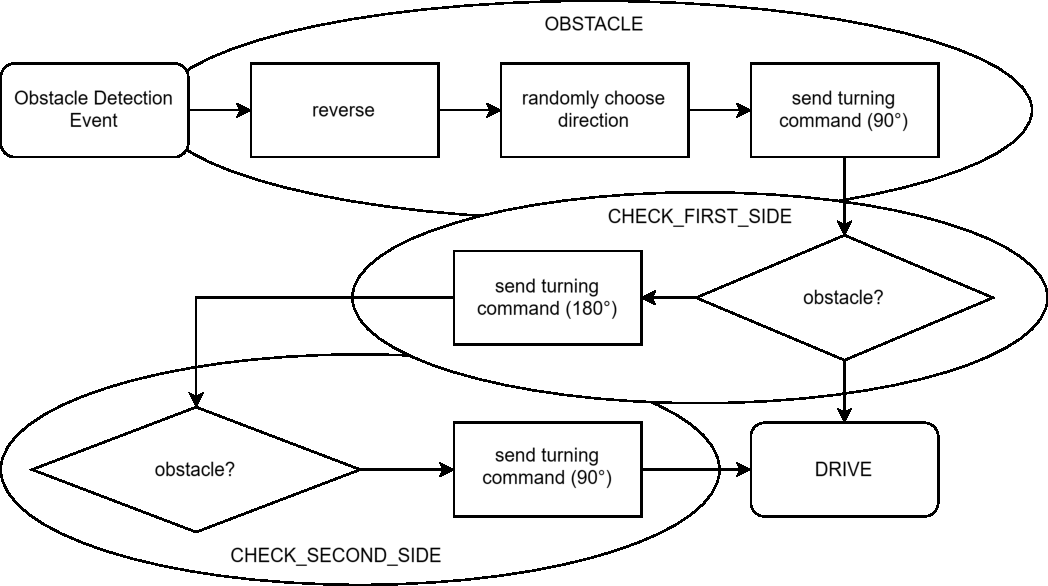
\includegraphics[scale=0.75]{obrazky-figures/wandering_obstacle_diagram.pdf}
	\caption{Algoritmus vyhýbání se překážkám}
	\label{fig:alg_obstacle}
\end{figure}

\verb|SCAN_START| je oproti předchozímu chování více obezřetné. Jeho originálním záměrem bylo hledat překážky, které zmizely z ultrazvukového senzoru (více o tomto jevu na straně~\pageref{implementation:ultrasonic}). Tato funkcionalita byla následně rozšířena a ve finální verzi probíhá skenování prostoru před robotem v pravidelných intervalech. Vzhledem k tomu, že se jedná o preventivní akci, nesnaží se vyhýbat překážkám přímo před robotem. Jeho cílem je nalézt překážky v blízkosti aktuální trajektorie robota. A v reakci na ně odklonit směr pohybu dále od nich. Pokud skenování nalezne překážku přímo před robotem, pokračuje v pohybu vpřed. Tím efektivně přenechává vyřešení tohoto problému \verb|OBSTACLE| stavu. Možné přechody do úvodního stavu skenování lze vyvodit z předchozího textu. Prvním je přijmutí varování o detekci zmizelé překážky od ultrazvukového senzoru. Druhým je pak pravidelný přechod ze stavu \verb|DRIVE|.

Algoritmu skenování je opět zobrazen na následujícím diagramu (obr:~\ref{fig:alg_scan}). Úhel hledání překážek je 90°. Celkem je provedeno šest čtení začínající na úhlu -45° a končící na +45°. Získaná data jsou následně interpretovány a je učiněna adekvátní reakce.

\begin{figure}[h!]
	\centering
	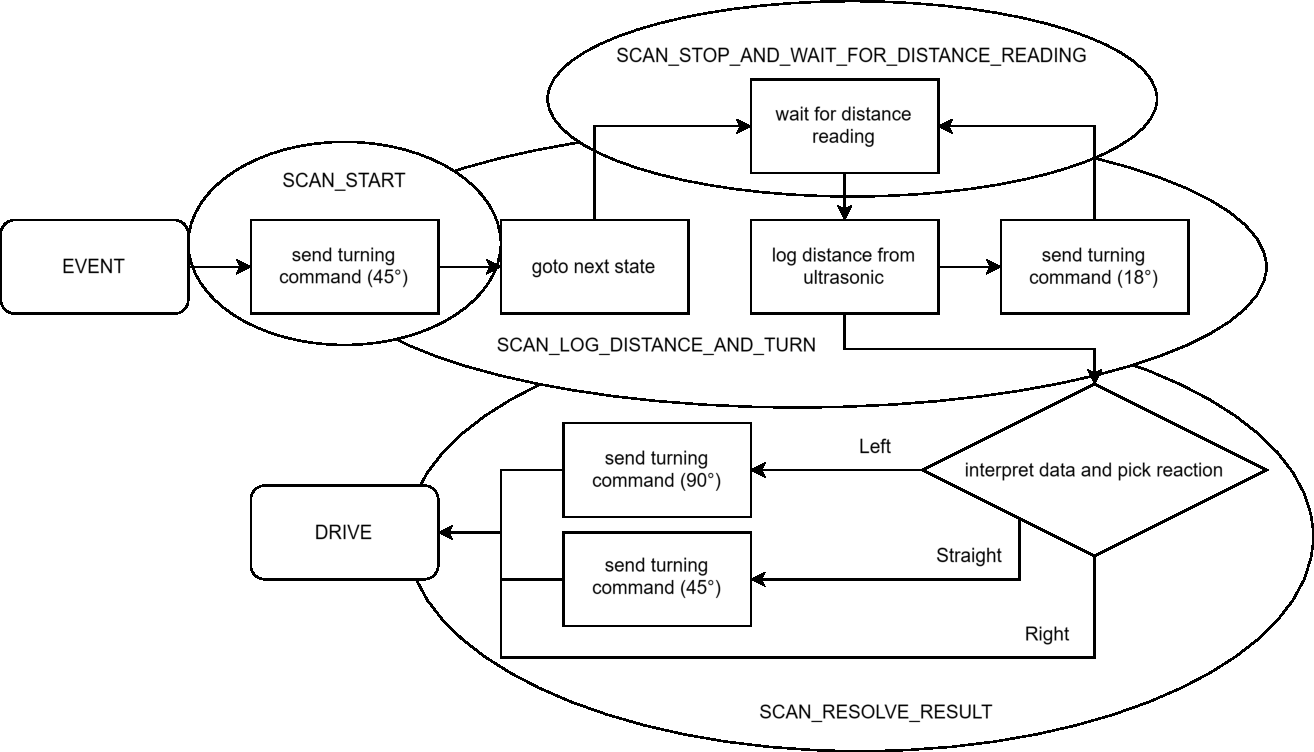
\includegraphics[scale=0.65]{obrazky-figures/wandering_scan_diagram.pdf}
	\caption{Algoritmus preventivního hledání překážek.}
	\label{fig:alg_scan}
\end{figure}

\subsection*{Sledování čáry}
Sledování čáry je v robotice známý úkol a na vyšších úrovních se v této disciplíně pořádají závody. Avšak v základním provedení se jedná o jednoduchý úkol. Tato funkcionalita je implementována hlavně z toho důvodu, že robot disponuje senzorem, který je k sledování čáry určený.

Implementace je provedena použitím konečného automatu. Použitý senzor je třícestný. Automat tedy bude obsahovat s $2^3$ stavů. Z tohoto počtu jsou dva stavy koncové a to 101, protože se jedná o nevalidní stav a 000 indikující ztrátu čáry. Mezi všemi ostatními lze navzájem přecházet. Následující stav se volí podle aktuálních hodnot senzorů. Přechodová logika byla následně obohacena o další podmínky s cílem reagovat na ztrátu čáry. To umožnilo následovat čáru s ostrými zatáčkami (pravý úhel a více). A také překonávat krátké přerušení v čáře. Zde je důležité zmínit, že tato funkcionalita byla testována hlavně v simulátoru a i tam má poměrně hodně nedostatků. 

\section{Spouštěcí soubory (Launch files)}
Každý uzel ve výsledném systému má k sobě vytvořený spouštěcí soubor. Ve většině případů se jedná o jednoduché soubory, jejichž úkolem je načtení a předání konfiguračního souboru spouštěnému uzlu. Někdy je vhodné umožnit uživateli při spouštění uzlu hodnotu parametru přepsat. Aby spouštěcí soubory toto umožnily, musí parametr explicitně definovat.
\begin{verbatim}
	ros2 launch lauch.py param_name:=value
\end{verbatim}
Ve složce \verb|ros2_ws/launch| se nachází hromadné spouštěcí soubory. Ty mají za úkol využít nižších spouštěcích souborů k nastartování větší části systému zároveň. Díky této hierarchické struktuře už není potřeba řešit předávání všech parametrů a lze se zaměřit jen na to důležité. Pokud jsou volány soubory, které parametry explicitně definují, lze je v tento moment přepsat, stejně jako by to udělal uživatel z příkazové řádky. Příkladem využití této funkcionality je řídící uzel \verb|wandering_node|. Pokud je tento uzel spuštěn manuálně, předpokládá se, že v systému žádný jiný řídící uzel neběží. Může tedy zahájit vykonávání hned po inicializaci, aniž by jeho příkazy kolidovaly s dalšími řídícími uzly. V případě, že je však volán jako součást hromadného spouštění, přepíše se výchozí hodnota parametru \verb|start_right_away| a všechny řídící uzly tak budou po inicializaci čekat na příkaz pro zahájení vykonávání.
\begin{verbatim}
IncludeLaunchDescription(
    launch_goal,
    launch_arguments={'start_right_away': 'false'}.items()
)
\end{verbatim}

Hromadné spouštěcí soubory startují mnoho uzlů zároveň. Běžným požadavkem je výměna několika málo uzlů za jiné. V takovém případě by bylo potřeba vytvořit druhý, převážně totožný soubor. K eliminaci tohoto problému slouží podmíněné spouštění. Jeho jednoduchou verzi využívá \verb|adeept_robot_launch.py|. V tomto případě slouží k rozhodnutí, který ze dvou uzlů určených k řízení motorů bude použit. Cílům spouštěcího souboru se do proměnné \verb|condition| přidá podmínka. Jedná se o speciální třídy (\verb|Ifcondition|, \verb|Unlesscondition|, \dots). V konstruktoru se jim předává true / false výraz. Jeho hodnotu lze získat například z parametru. Podmíněné spouštění může být i komplexnější, a to v kombinací s \verb|PythonExpression|. Tato třída je použita v souboru \verb|gazebo_simulation_launch.py|, kde se porovnáním hodnoty parametru určuje, který svět bude spuštěn.
\begin{verbatim}
IncludeLaunchDescription(
    launch_goal,
    condition=IfCondition(
        PythonExpression([
            '"', world_select_val, '"', ' == "wandering"'
        ])
    )
)
\end{verbatim}

Komplexnější spouštěcí soubory často potřebují větší kontrolu nad tím, kdy dojde ke provedení jednotlivých cílů. V případě, že je potřeba pouze opozdit provedení některého z cílů lze využít \verb|TimerAction|. Jedná se o třídu, která spustí daný cíl až po uplynutí předem stanoveného časového intervalu. Ve finální verzi systému byla tato funkcionalita nahrazena lepšími přístupy. Jako příklad, kde byla v průběhu vývoje použita je soubor \verb|diff_drive_launch.py|. Sloužila k zpoždění \uv{spawn} ovladače až po dokončení inicializace zbytku \verb|ros2_control|.
\begin{verbatim}
TimerAction(
    period=10.0,
    actions=[launch_goal]
)
\end{verbatim}

K přesnějšímu řízení slouží obsluha událostí (event handler). Ta umožňuje detailnější kontrolu nad tím, kdy dojde k vykonání jednotlivých cílů. Typickými událostmi jsou spuštění a ukončení procesu, případně, pokud se jedná o lifecycle uzly, také reakce na přechody do konkrétních stavů. Obsluha událostí je využita přímo v balíku Gazebo simulace v~souboru \verb|gazebo_world_launch.py|. Je zde celý řetěz těchto obsluh, které postupně spustí simulaci, přeloží \verb|xacro| model na \verb|urdf|, \uv{spawnou} jej do simulace a po jejím ukončení ještě uklidí vygenerovaný \verb|urdf|.

\begin{verbatim}
RegisterEventHandler(
    OnProcessStart(
        target_action=simulator,
        on_start=convert_xacro
    )
)
\end{verbatim}

\section{Model robota} \label{implementation:model}
Model robota slouží k předání informace o jeho struktuře, vzhledu a fyzikálních vlastnostech dalším částem ROS2 systému. Formát pro definici modelu, který ROS2 používá je \verb|urdf|. Většina nástrojů však nepracuje přímo s definicí v \verb|urdf| formátu, ale získává tyto informace z \verb|/tf| subsystému. Zpracování, interpretaci a následné odesílání informací o aktuálním stavu robota zajišťuje \verb|robot_state_publisher|. Jedná se o oficiální ROS2 uzel. Vstupem tohoto uzlu je \verb|urdf| model robota. Prvním výstupem je odesílání statických i dynamických transformací do \verb|/tf| systému. Aby mohl odesílat dynamické transformace musí mít informaci o~aktuálních natočení kloubů. Ty získává posloucháním \verb|joint_states| topicu (obr:~\ref{fig:rviz_robot_desc}).

Druhým výstupem tohoto uzlu je topic \verb|robot_description|. Jeho obsahem je celý \verb|urdf| popis, odeslaný jakožto string zpráva.

\begin{figure}[h!]
	\centering
	\begin{minipage}[c]{0.45\textwidth}
		\centering
		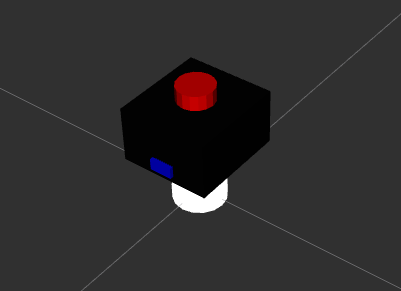
\includegraphics[scale=0.45]{obrazky-figures/robot_description_no_joint_states.png}
	\end{minipage}%
	\begin{minipage}[c]{0.55\textwidth}
		\centering
		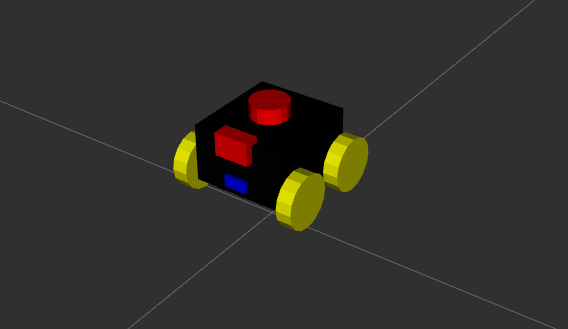
\includegraphics[scale=0.4]{obrazky-figures/robot_description_joint_states.png}
	\end{minipage}
	\caption[Zobrazení popisu robota v nástroji Rviz]{Zobrazení dat z robot\_state\_publisheru v nástroji Rviz. Levý obrázek zobrazuje pouze statické tranformace (joint\_states topic je prázdný), pravý pak celý model}
	\label{fig:rviz_robot_desc}
\end{figure}

\subsection*{Tvorba modelu}
Jak už bylo řečeno, základní formát používaný k popisu modelů je \verb|urdf|. ROS2 využívá také druhý, rozšiřující formát \verb|xacro|. Cílem \verb|xacra| je vyřešit některé neduhy čistého \verb|urdf| a usnadnit tak vývojářům psaní popisů robotů. Tato práce používá k popisu robota \verb|xacro| formát.

Následující blok kódu demonstruje využití téměř všech možností \verb|xacra| na jednom místě.
V čistém \verb|urdf| se velmi často opakuje téměř totožná definice \verb|<link>| elementu. Jedná se o~zdlouhavý zápis s minimálními změnami. Následující blok kódu vytváří makro, které umožní zkrátit tuto nepřehlednou a na chyby náchylnou sekci na jednořádkové zavolání makra. Pro zvýšení znovupoužitelnosti, využívá toto makro také parametry. Ty jsou předány v místě použití makra. Díky nim může být makro obecnější, a tedy použitelné na více místech. Poslední parametr ukazuje také možnost nastavení výchozí hodnoty parametru. Parametry lze využít také v matematických výrazech. Manuální výpočet matice setrvačnosti pro každý \verb|<link>| element je zbytečně složité a opět náchylné na chyby. Použití matematického výrazu, který se sám vyhodnotí podle hodnot předaných parametry je výrazně lepší a pohodlnější přístup.

\begin{algorithm}[h!]
	\label{}
	\caption{\textsc{Macro with params}}
	
	\DontPrintSemicolon
	\SetAlgoNoLine
	\SetAlgoNlRelativeSize{-1}
	\SetNlSty{}{}{:}
	\SetNlSkip{-1.1em}
	
	\BlankLine \Indp\Indpp
	
	\texttt{<xacro:macro name="box\_link" params="name mass x y z material:=red">}\;
	\Indp\Indp
	\texttt{<link name="\${name}">}\;
	\Indp\Indp
	\texttt{<inertial>}\;
	\Indp\Indp
	\texttt{<mass value="\${mass}" />}\;
	\texttt{<inertia ixx="\${(1/12) * mass * (y*y+z*z)}" ixy="0.0" ixz="0.0"}\;
	\Indp\Indp
	\texttt{\hspace{2.6em}iyy="\${(1/12) * mass * (x*x+z*z)}" iyz="0.0"}\;
	\texttt{\hspace{2.6em}izz="\${(1/12) * mass * (x*x+y*y)}" />}\;
	\Indm\Indm
	\Indm\Indm
	\texttt{</inertial>}\;
	\texttt{<visual>}\;
	\Indp\Indp
	\texttt{<geometry>}\;	
	\Indp\Indp
	\texttt{<box size="\${x} \${y} \${z}"/>}\;
	\Indm\Indm
	\texttt{</geometry>}\;
	\texttt{<material name="\${material}"/>}\;
	\Indm\Indm
	\texttt{</visual>}\;
    \begin{center}
	\texttt{\vdots}
	\end{center}
	
\end{algorithm}

Popis robota v \verb|xacro| formátu nelze použít jako přímou náhradu \verb|urdf|, ale musí být nejprve přeložen. K tomu slouží následující příkaz. Při překladu dojde k svázání zdrojových souborů dohromady, nahrazení a vyhodnocení maker, matematických výrazů a parametrů.
\begin{verbatim}
	xacro in.xacro > out.urdf
\end{verbatim}

Nakonec by bylo ještě dobré zmínit, že do definic modelů lze vkládat aplikačně specifické tagy. Příkladem je \verb|<gazebo>| nebo \verb|<ros2_control>| tag. Nástroje interpretující \verb|urdf| definice s tímto počítají a pokud narazí na neznámý tag, tak jej prostě přeskočí.

\newpage
\section{Uživatelské rozhraní}
Vytvořené uživatelské rozhraní využívá knihovnu Qt, konkrétně její Python verzi PyQt5.\footnote{\url{https://pypi.org/project/PyQt5/}} Rozhraní jako takové je odděleno od ostatních řídících funkcionalit. Pouze zajišťuje zobrazování informací získatelných z topiců a odesílání příkazů ostatním uzlům. Zbytek ROS2 systému je tedy plně ovladatelný z prostředí příkazové řádky. Co se týče implementace, tak ROS2 i QT mají svůj vlastní execution loop. To vytváří problém, protože pokud jeden z~nich neběží, tak daná část nefunguje. Jedním z možných řešení je použití více procesů. To však vede na problémy se synchronizací. Lepší a také použitý přístup je řídit oba cykly manuálně. 
\begin{verbatim}
	while stoping_variable:
	    rclpy.spin_once(node, timeout_sec=0.001)
	    app.processEvents()
\end{verbatim}
Tímto způsobem můžou obě části řešit svou vlastní funkcionalitu a zároveň volat funkce té druhé. ROS2 část zajišťuje komunikaci se zbytkem systému. Získává z něj data, které předává Qt části. Qt část zajistí jejich zobrazení a reakce na uživatelské příkazy. Příkazy pro další uzly pak přeposílá zpět do ROS2 části, které je odešle do systému.

\begin{figure}[h!]
	\centering
	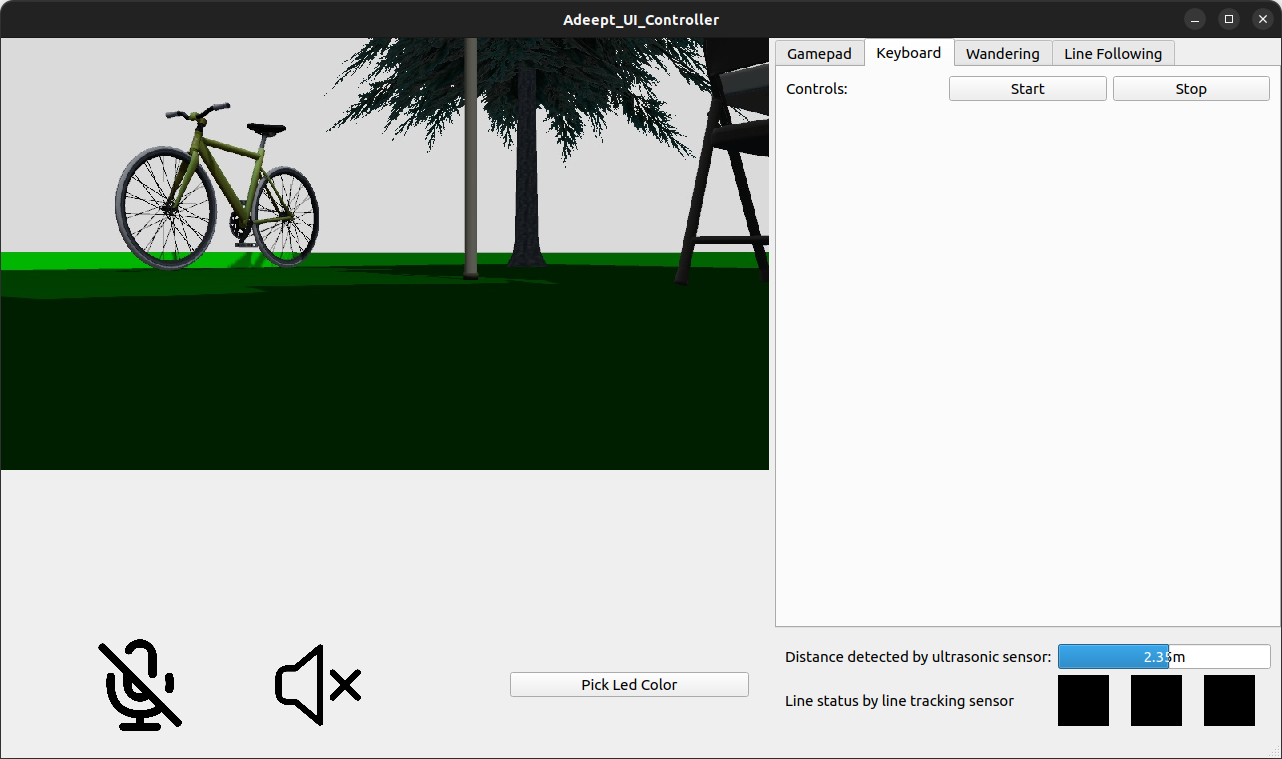
\includegraphics[scale=0.3]{obrazky-figures/ui.png}
	\caption{Uživatelské rozhraní}
	\label{fig:ui}
\end{figure}

\chapter{Nástroje související s ROS2}
Tato kapitola se již odchýlí od čistého ROS2 systému a původního zadání práce. Jejím cílem je představit související nástroje, které buď usnadňují vývoj nebo výrazným způsobem rozšiřují schopnosti výsledného systému.

\section{Gazebo simulátor}
Použití simulátoru při vývoji softwaru na řízení robotů je časté a užitečné. Umožňuje vyvíjet software i bez fyzického robota, případně testovat funkcionalitu bez vlivů reálného světa. Tato práce využívá novou \verb|ignition| větev Gazebo simulátoru.\footnote{\url{https://github.com/gazebosim}}

\subsection*{Světy}
Před tím než lze začít využívat výhody simulátoru, je nejprve potřeba vytvořit model robota a světy ve kterých se bude pohybovat. Nativním formátem, který Gazebo využívá je \verb|sdf|. V této práci je \verb|sdf| použito k definici světů. Více o struktuře světů na straně \pageref{theory:gazebo}. Konkrétně byly vytvořeny tři ukázkové světy.

\begin{itemize}[leftmargin=*]
	\item{Wandering}
\end{itemize}
\vspace*{-0.5em}
Primární testovací svět pro bloudění, mapování a navigaci.

\begin{itemize}[leftmargin=*]
	\item{Garden}
\end{itemize}
\vspace*{-0.5em}
Vizuálně nejhezčí svět. Načítá modely z fuel knihovny.

\begin{itemize}[leftmargin=*]
	\item{Line Tracking}
\end{itemize}
\vspace*{-0.5em}
Testovací svět pro sledování čáry. Používá \verb|<mesh>| tag pro načtení objektu vytvořeného v~Blenderu.

\subsection*{Definice modelu}
Pro definice modelů existuje několik použitelných formátů. První možností je využít stejně jako pro světy formát \verb|sdf|. Tímto způsobem lze zapsat definici modelu ve stejném souboru jako zbytek světa. Pokud se jedná o komplexnější definici lze ji zapsat externě a vložit od světa pomocí \verb|<include>| tagu. Z důvodu kompatibility se zbytkem ROS2 systému umožňuje Gazebo použít také \verb|urdf| potažmo \verb|xacro| soubory. Modely definované v \verb|urdf| se do světa nevkládají přímo, ale \uv{spawnují} se až po spuštění simulace. Slouží k tomu Gazebo služba jménem \verb|/world/world_name/create| a příkaz \verb|ign service|.

Klasický model (viz strana: \pageref{implementation:model}) definuje vizuální a fyzikální vlastnosti robota. Tato definice struktury je pro většinu nástrojů dostačující. Rozdílem je simulátor, který potřebuje získat dodatečné informace o tom, jaké fyzické komponenty jednotlivé elementy modelu reprezentují. K tomu slouží \verb|<gazebo>| tag. Jeho obsahem jsou \verb|sdf| definice. Typicky se do něj vkládají \verb|<sensor>| a \verb|<plugin>| tagy (viz strana \pageref{theory:gazebo}). 

Při převodu fyzického robota do simulátoru bylo potřeba vyřešit několik problémů. Jedním z nich je ten, že Gazebem podporované senzory jsou typicky ty komplexnější jako lidar a hloubkové kamery. Naopak jednodušší snímače použité na demonstračním robotovi nejsou nativně implementovány. Ultrazvukový senzor vzdálenosti je tedy ve výsledném modelu nahrazen lidarem. Aby se jeho fungování více blížilo referenčnímu senzoru, byl omezen úhel měření na 15° a počet vysílaných paprsků na tři. Modul pro sledování čáry je pak realizován pomocí tří kamer. Každá s rozlišením jeden pixel. Získané RGB hodnoty následně zpracovává pomocný uzel.

\subsubsection*{ROS Gazebo bridge}
Krása Gazebo simulátoru je jeho provázání s ROS2 systémem. Díky tomu lze použít stejné řídící uzly pro reálného i simulovaného robota. Gazebo vnitřně používá podobný systém topiců a zpráv jako ROS2. Pomocí oficiálního nástroje \verb|ros_gz_bridge| lze přemostit komunikaci mezi ROS2 a Gazebem. Spouští se pomocí příkazu:
\begin{verbatim}
	ros2 run ros_gz_bridge parameter_bridge 
	/topic_name@ros_msg_type@gazebo_msg_type
\end{verbatim}
Pro hromadnější použití lze předat bridge uzlu konfigurační soubor s definicí více topiců, pro přemostění.
\begin{verbatim}
	- ros_topic_name: "ros_chatter"
	gz_topic_name: "gz_chatter"
	ros_type_name: "std_msgs/msg/String"
	gz_type_name: "gz.msgs.StringMsg"
	direction: IGN_TO_ROS  # BIDIRECTIONAL or ROS_TO_IGN
\end{verbatim}

\newpage
\subsubsection*{Zajištění kompatibility}
Ve většině případů stačí k zajištění kompatibility čisté přemostění topiců mezi Gazebem a~ROSem. Ale existují také speciální případy, kdy je potřeba data nějakým způsobem upravit, aby blíže odpovídaly reálnému robotu. 

\begin{itemize}[leftmargin=*]
	\item{Kamera}
\end{itemize}
\vspace*{-0.5em}
Most pro přenos obrazových dat využívá na ROS2 straně zprávy typu Image. Ale jak bylo podrobněji probráno v sekci o fyzické kameře (str:~\pageref{implementation:camera}). Výstup z uzlu pro její ovládání je ve formátu CompressedImage. Proto musí být data vycházející ze simulátoru přetypovány, aby byla zajištěna jejich kompatibilita.

\begin{itemize}[leftmargin=*]
	\item{Sledování čáry}
\end{itemize}
\vspace*{-0.5em}
Jak bylo řečeno výše, Gazebo nemá nativní podporu senzoru pro sledování čáry. Výstup ze simulátoru je tedy ve formátu tří Image zpráv, každá obsahující jeden RGB pixel. Vzhledem k tomu, že se jedná o tři samostatné zprávy, musí být nejprve seskupeny podle časových značek. Poté jsou získaná data převedena na binární hodnotu reprezentující viditelnost čáry. To je provedeno zkombinováním RGB složek pixelu na jedu hodnotu ve stupních šedi (grayscale). Na ni lze následně aplikovat prahování (thresholding) a získat tak výsledné rozhodnutí o viditelnosti čáry.

\begin{itemize}[leftmargin=*]
	\item{Měření vzdálenosti}
\end{itemize}
\vspace*{-0.5em}
Ultrazvukový senzor je v simulátoru proveden pomocí lidaru. Je tedy potřeba zkombinovat data ze všech tří paprsků do výsledné vzdálenost. Uzel ovládající fyzický senzor, také odesílá dodatečné varování ohledně detekování překážek. Proto je nutné doplnit také tuto funkcionalitu.

\begin{itemize}[leftmargin=*]
	\item{Servo}
\end{itemize}
\vspace*{-0.5em}
Uzel pro ovládání fyzického serva používá akční server. Tento simulovaný musí z důvodu kompatibility dělat totéž.

\begin{itemize}[leftmargin=*]
	\item{Lidar}
\end{itemize}
\vspace*{-0.5em}
V případě lidaru jsou data z simulátoru přímo kompatibilní s ROS2 a tak jedinou úpravou je přemapování jména topicu.

\begin{itemize}[leftmargin=*]
	\item{Motory, odometrie, pozice kloubů}
\end{itemize}
\vspace*{-0.5em}
Části řešící pohyb a odometrii robota využívají ros2\_control. Podrobněji popsáno v následující sekci. Komunikaci mezi ROS2 a simulátorem v tomto případě zajišťuje ros2\_control plugin pro Gazebo simulátor. Na rozdíl od reálného robota je v simulátoru odometrie získávána z enkodérů motorů kol. 

\newpage
\section{Ros2 control}
Ros2 control je framework implementující teorii řízení.\footnote{\url{https://github.com/ros-controls}} V sekci o ovládání komponent byl představen uzel, který ovládá stejnosměrné motory s cílem realizovat diferenciální pohyb robota. Tvorba vlastního uzlu k tomuto účelu je zcela validní přístup. Problém je v tom, že podobný uzel bude potřebovat každý mobilní robot. A proto existuje ros2 control, který má za cíl zjednodušit tvorbu řídících systémů. \cite{ros2_control_documentation}

\subsection*{Controller manager}
Je hlavní řídící jednotkou, která zajišťuje navázání ovladačů (controllers) a hardwarových pluginů (drivers). Manager se spouští pomocí uzlu \verb|ros2_control_node|. Jako první krok po spuštění potřebuje získat informace o robotovi, kterého bude ovládat. Ty hledá v \\ \verb|robot_description| topicu. Konkrétně jej zajímá tag \verb|<ros2_control>|. Z něj získá seznam kloubů a hardwarových rozhraní, kterými tyto klouby disponují. Příkazové rozhraní \verb|command_interface| slouží k posílání dat směrem k hardwaru. Typicky se jedná o nastavení rychlosti (velocity) otáčení motoru. Stavové rozhraní \verb|state_interface| pak slouží k~získávání informací od komponenty zpět do ROS2 systému. Příkladem může být výstup enkodéru motoru. Dalším inicializačním krokem je zpracování konfiguračního souboru. Ten obsahuje seznam použitelných ovladačů a jejich nastavení. V tento moment bude manager čekat na spuštění některého z ovladačů definovaných v konfiguračním souboru, aby mohlo dojít k~jeho navázání na kompatibilní hardwarové rozhraní. Tímto krokem je vše připraveno a může započít ovládání robota. \cite{ros2_control_documentation} 

Robot použitý v této práci se pohybuje diferenciálním způsobem. Jako ovladač je tedy použit existující \verb|differential drive controller|. Ten zajišťuje příjem \verb|cmd_vel| příkazů a následné výpočty týkající se kinematiky. Hardwarový plugin sloužící k ovládání motorů je implementován v rámci této práce. Jeho hlavním úkolem je ovládání GPIO vývodů.

\subsection*{Model}
Jak už bylo řečeno, Controller manager používá \verb|urdf| definici k získání informací o použitém robotu a hardwarových pluginech určených k jeho řízení. Proto je potřeba tuto definici rozšířit o \verb|<ros2_control>| tag. Do jeho těla se umisťují \verb|<hardware>| a \verb|<joint>| tagy. První zmíněný slouží k výběru konkrétního pluginu a nastavení jeho parametrů. Druhý pak přiřazuje zvolenému pluginu jednotlivé klouby, které bude mít za úkol ovládat. Obsahem \verb|<joint>| tagu jsou také definice rozhraní, kterými kloub disponuje. \cite{ros2_control_documentation}

\subsection*{Hardwarový plugin}
Hardwarové pluginy, jak z názvu vyplývá, jsou části kódu, které budou v ros2\_control ekosystému zajišťovat komunikaci s komponentami. Na rozdíl od controlerů, u kterých lze často využít existující implementace, protože se požadované funkcionality opakují. U~hardwarových pluginů to neplatí, protože existuje mnoho různých komponent, s různými způsoby ovládání. Na psaní pluginů se používá jazyk C++. Struktura kódu je stejná jako lifecyle uzly v ROS2. Jedná se o speciální přístup, který definuje sadu metod sloužících k inicializaci a destrukci objektu (obr:~\ref{fig:lifecycle_diagram}).

\begin{figure}[h!]
	\centering
	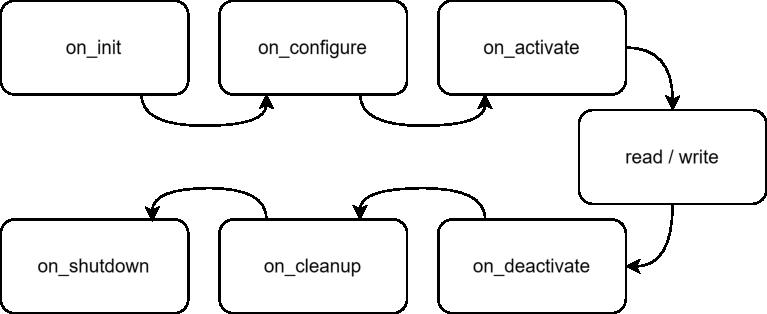
\includegraphics[scale=0.8]{obrazky-figures/ros2_control_wh_plugin_transitions.pdf}
	\caption{Běžný postup volání lifecycle funkcí}
	\label{fig:lifecycle_diagram}
\end{figure}

\newpage
\begin{itemize}[leftmargin=*]
	\item{\verb|on_init|}
	\vspace*{-0.5em}
	\begin{itemize}
		\item{načtení parametrů definovaných v urdf modelu}
		\item{kontrola, že klouby zadané v urdf odpovídají očekávání}
	\end{itemize}
	\item{\verb|on_configure / on_cleanup|}
	\vspace*{-0.5em}
	\begin{itemize}
		\item{připravení a nastavení hardwaru}
		\item{například výběr gpio pinů, nastavení jejich směru, inicializace PWM}
	\end{itemize}
	\item{\verb|on_activate / on_deactivate|}
	\vspace*{-0.5em}
	\begin{itemize}
		\item{}
	\end{itemize}
	\item{\verb|export_state_interfaces| / \verb|export_command_interfaces|}
	\vspace*{-0.5em}
	\begin{itemize}
		\item{nabídne rozhraní definované v urdf a inicializované v pluginu k spárování s ovladači}
	\end{itemize}
	\item{\verb|read|}
	\vspace*{-0.5em}
	\begin{itemize}
		\item{získává hodnoty z hardwaru a ukládá je do vnitřních proměnných, aby se jejich hodnoty mohly dostat k ovladačům}
	\end{itemize}
	\item{\verb|write|}
	\vspace*{-0.5em}
	\begin{itemize}
		\item{podle hodnot z vnitřních proměnných zasílá příkazy hardwarovým komponentům}
	\end{itemize}
\end{itemize}

V rámci této práce byl vytvořen plugin pro řízení stejnosměrných motorů. Jedná se o~podobný princip jako v samostatném uzlu (viz str: \pageref{implementation:motors}). Jediným podstatným rozdílem je použití jiné knihovny, jazyka C++, lifecycle metod a potřeba generovat si PWM manuálně. Pro ovládání GPIO pinů byla použita knihovna libgpiod.\footnote{\url{https://git.kernel.org/pub/scm/libs/libgpiod/libgpiod.git/about/}}

\subsection*{Controllers}
Ovladače se definují pomocí konfiguračního \verb|yaml| souboru. Ten následuje stejná pravidla, jako konfigurace pro kterýkoli jiný ROS2 uzel. Nejprve se zadávají parametry pro samotný \verb|controller_manager|. Zde se volí ovladače, které bude možné načíst. Dále pak následují specifické konfigurace pro ovladače. \cite{ros2_control_documentation}

\subsection*{Integrace ros2 control s Gazebo simulátorem}
Slouží k tomu balíček \verb|gz_ros2_control|. Struktura ros2\_control zůstává i pro simulátor stále stejná. Hlavní změnou je výměna pluginů v \verb|urdf| definici. Hardwarový plugin bude ovládat simulovaného robota a proto musí být vyměněn. Aby mohl interagovat se simulátorem musí být přidán nový plugin pro Gazebo. Zjednodušením oproti použití na fyzickém robotu je to, že plugin pro Gazebo zajistí spuštění Controller manageru a není jej potřeba zapínat externě.

\begin{algorithm}[h!]
	\label{}
	\caption{\textsc{Načtení pluginu a předání konfiguračního souboru}}
	
	\DontPrintSemicolon
	\SetAlgoNoLine
	\SetAlgoNlRelativeSize{-1}
	\SetNlSty{}{}{:}
	\SetNlSkip{-1.1em}
	
	\BlankLine \Indp\Indpp
	
	\texttt{<plugin filename="control-system.so" name="GazeboSimROS2ControlPlugin">}\;
	\Indp
	\texttt{<parameters>\$(find package\_name)/config/controllers.yaml</parameters>}\;
	
\end{algorithm}

\section{Navigace a mapování}
Jádrem mapování a navigace jsou použité knihovny \verb|slam_toolbox| a \verb|navigation2|. Aby fungovaly, musí jim podkladový systém poskytnout potřebné informace. Většina práce ke zprovoznění mapování a navigace spočívá právě v této přípravě.

\subsubsection*{Model}
Obě knihovny hojně využívají \verb|/tf| subsystém. Z něj získávají informace o struktuře a transformacích robota. Podrobněji se o \verb|/tf| mluví na straně \pageref{theory:tf} a o modelech na straně \pageref{implementation:model}.

\subsubsection*{Odometrie}
Druhým krokem k mapování a lokalizaci je získání aktuálních souřadnic, orientace a rychlosti robota. K tomu slouží odometrie (obr:~\ref{fig:rviz_odom}). Odometrická dala lze získat několika způsoby. Jedním z často používaných a také poměrně přesných přístupů je využití dat získaných z~enkodérů motorů kol. Ty lze přepočítat na vzdálenost, kterou urazily jednotlivá kola diferenciálního podvozku. \cite[str:~171-172]{mobilní_roboty} Vzhledem k tomu, že použitý robot nedisponuje motory s enkodéry, byl v této práci využit druhý přístup. Tím je zpracování dat získaných z~imu senzoru. Integrací dat z akcelerometru a gyroskopu lze získat aktuální pozici a natočení vůči počátku. Nevýhodou tohoto přístupu je jeho menší přesnost a akumulace chyb vedoucí k postupnému vzdalování předpokládané pozice od reality. Postupná akumulace chyby v~odometrii však vzniká u všech přístupů. A proto části ROS2 systému realizující mapování a navigaci s touto skutečností počítají. V této práci odometrii počítá uzel \verb|imu_node|, který výsledná data odesílá jako odom rám do tf subsystému. 

\begin{figure}[h!]
	\centering
	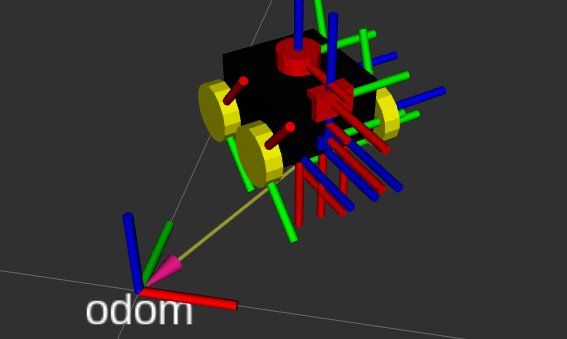
\includegraphics[scale=0.6]{obrazky-figures/odom.png}
	\caption[Zobrazení transformací a odometrie v nástroji Rviz]{Zobrazení robota včetně jeho transformačních rámů v Rviz, fixed\_frame je nastaven na odom a robot se tedy může pohybovat oproti počátku souřadného systému}
	\label{fig:rviz_odom}
\end{figure}

\subsubsection*{Mapování}
Posledním krokem k úspěšnému mapování je získání dat o okolním prostředí. To zajišťuje lidar senzor umístěný na robotu. Aby bylo možné data získané z lidaru použít, musí existovat transformace mezi rámem lidaru a base frame robota. Pokud je lidar součástí definice modelu, postará se o tuto transformaci \verb|robot state publisher|.

Mapování jako takové zajišťuje perfektní knihovna \verb|slam_toolbox|.\footnote{\url{https://github.com/SteveMacenski/slam_toolbox}} Jedná se o komplexní soubor nástrojů souvisejících se SLAM. \\ Tato práce využívá \verb|async_slam_toolbox_node|. Jedná se o online async mapování. Online znamená, že uzel pracuje nad aktuálními daty, knihovna totiž umožňuje také tvorbu mapy z předem zaznamenané historie. Async pak zajišťuje zpracování vždy nejnovějších dat, což zlepšuje latenci, ale může vést k přeskočení některých scanů. Vzhledem k tomu, že slam je komplexní problém, existuje mnoho nastavitelných parametrů. Ty se předávají při spouštění pomocí konfiguračního souboru. V demonstračních příkladech poskytnutých \verb|slam_toolboxem| se nahází ukázkový konfigurační soubor, který byl jen s menšími modifikacemi využit i v této práci. Hlavní změnou je zvýšení rozlišení vytvářené mapy. Vývojáři knihovny předpokládají její využití v průmyslu a základní hodnoty tedy počítají s tím, že robot je větší a pohybuje se ve velkých halách. Uzel odesílá výslednou mapu ve standardním formátu \verb|nav_msgs/OccupancyGrid| do \verb|/map| topicu (obr:~\ref{fig:rviz_slam_map}).

\begin{figure}[h!]
	\centering
	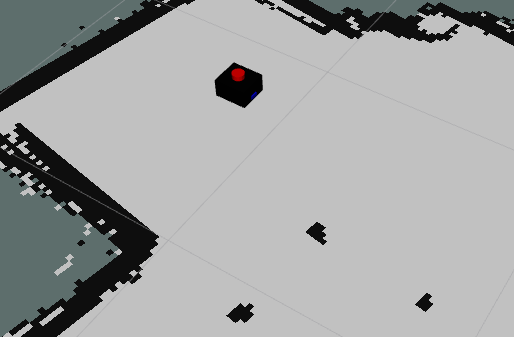
\includegraphics[scale=0.7]{obrazky-figures/slam.png}
	\caption{Mapa vytvořená slam toolboxem zobrazená v nástroji Rviz}
	\label{fig:rviz_slam_map}
\end{figure}

\subsubsection*{Navigace}
Pro navigaci byla využita knihovna Navigation 2 (viz strana \pageref{theory:nav2}).\footnote{\url{https://github.com/open-navigation/navigation2}} 
Z vnějšího pohledu uzly Nav2 poslouchají topicy \verb|/scan| (lidar data), \verb|/map| (slam mapa) a transformace z tf systému. Primárně vztah mezi \verb|map|, \verb|odom| a lidar rámem. Zobrazitelným výstupem je několik nákladových map (costmap) (obr:~\ref{fig:rviz_costmap}). Jedná se o upravenou mapu z \verb|/map| topicu obohacenou o ceny jednotlivých polí. Tyto ceny jsou používány plánovacím serverem k určení optimální cesty k cíli. Příkaz pro zahájení navigace je přijímán akčním serverem se jménem \verb|/navigate_to_pose|. 

\begin{figure}[h!]
	\centering
	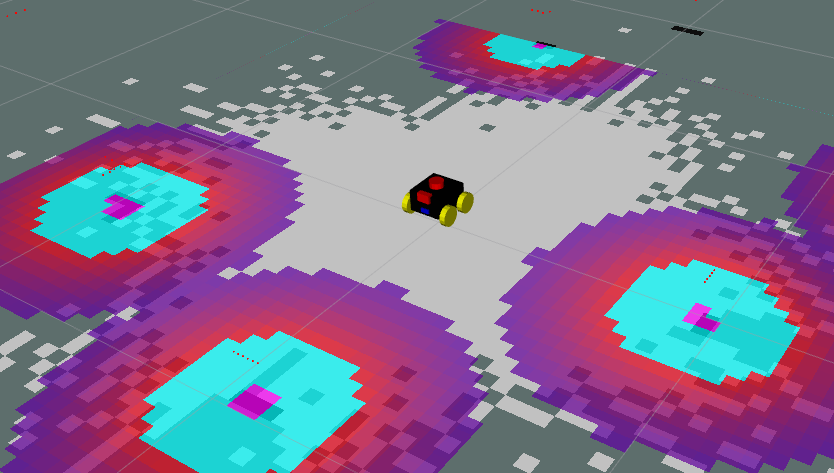
\includegraphics[scale=0.7]{obrazky-figures/nav2.png}
	\caption{Slam mapa překrytá lokální navigation 2 costmapou v nástroji Rviz}
	\label{fig:rviz_costmap}
\end{figure}

Spouštění Nav2 systému vyžaduje nastartování a nakonfigurování většího množství uzlů. Pomocí konfiguračních souborů může uživatel výrazně ovlivnit chování celého Nav2. Kromě toho, že obsahuje velké množství parametrů, umožňuje také vyměňovat řídící pluginy. V~balíku \verb|nav2_bringup| se nachází ukázkové spouštěcí a konfigurační soubory. Ty byly poupraveny a použity v této práci. Největší zásahy do konfigurace jsou motivovány cílem zprovoznit navigaci i přes limitace použitých motorů (viz strana~\pageref{implementation:motors}). Z těchto důvodů byly v~konfiguraci vyměněny dva pluginy. 

Tím prvním je ovladač pro řízení pohybu. Výchozí \verb|DWB Controller| realizuje otáčení robota jízdou po oblouku. Jak už je známo, s tímto přístupem má použitý hardware problém. Proto byl vyměněn za \verb|Rotation Shim Controller|. Ten zajišťuje, že robot se nejprve otočí ve směru plánované trajektorie a až pak zahájí pohyb vpřed. Pokud se odchýlí z~tohoto směru, dojde k zastavení a proběhne korekce. Pohyb, v momentě kdy je robot správně natočený, realizuje pomocný pod plugin. Tím je ve výchozím stavu \\ \verb|RegulatedPurePursuitController|. Druhým vyměněným pluginem je plánovač trasy. Nakonec byl použit \verb|Smac 2D Planner|. Zde nemám objektivní důvod pro tuto volbu. Ze subjektivního pohledu mi přišly jeho trasy vhodnější, protože obsahují menší počet zbytečných křivek, se kterými má robot problémy.

Kromě výměny pluginů byly v konfiguraci změněny také některé parametry. Navigace v~podání Nav2 je rozvážná a přesná. Pro tento přístup však potřebuje robota, který se dokáže pohybovat pomalu a~plynule. Běžné rychlosti, které Nav2 používá ve složitějších částech trasy, jsou okolo 0.05 m/s případně 0.2 rad/s. A zde nastává problém, protože použitý robot takové rychlosti nedokáže vyvinout. Minimální rychlost, která zajistí pohyb, je okolo 0.2 m/s. V konfiguraci lze naštěstí nastavit minimální rychlosti, které budou uzly Nav2 používat. Poslední sadou změn jsou úpravy rozměrů. Stejně jako u slam konfigurace je robot menší a pohybuje se v menších prostorech. Byla proto upravena velikost stopy robota, cíle a inflation vzdálenosti. Ty jsou přidány okolo překážek a ovlivňují ceny polí při plánování trasy.

Navigaci se nakonec podařilo zprovoznit. Jak už bylo několikrát zmíněno, Nav2 je komplexní systém a aby byla navigace v kombinaci s tímto robotem perfektní vyžadovala další ladění. V aktuální verzi má několik nedostatků (při inicializaci se na pár vteřin rozpadne tf strom, a po jejím dokončení se občas nezačnou publikovat costmapy), které však neovlivňují její fungování. Co se týče ovládání, tak všechny vstupní i výstupní data z Nav2 jsou posílána přes ROS2. Bylo by tedy možné implementovat ovládání do vlastního uživatelského rozhraní. Desktop verze ROS2 však obsahuje nástroj Rviz. Ten umožňuje zobrazování map i~zasílání příkazů. V kombinaci s jeho dalšími funkcemi je jednoznačně nejlepší možností pro uživatelskou interakci s Nav2.

\section*{Instalace}
K usnadnění zprovoznění výsledného systému byl vytvořen instalační skript \verb|setup.sh|. Jeho použití a další kroky jsou popsány v \verb|readme.md| souboru.

\chapter{Závěr}
Cílem práce bylo vytvořit ROS2 systém pro ovládání robota Adeept AWR 4WD a demonstrovat na něm možnosti ROS2. Tohoto cíle bylo úspěšně dosaženo. Vytvořený systém je rozdělen na dvě části provozované distribuovaně na robotu a stacionárním zařízení. První část, běžící na Raspberry Pi, realizuje interakci s komponentami robota. Pro každou komponentu byl implementován uzel, který zpřístupňuje její funkcionalitu ostatním částem ROS2 systému. Druhá část, běžící na stacionárním zařízení, zajišťuje řízení robota jako celku. Prvním řídícím režimem je manuální ovládání pomocí klávesnice nebo ovladače. Druhým režimem je automatické bloudění robota po místnosti s vyhýbáním se překážkám. Nad uzly byl implementován systém konfiguračních a spouštěcích souborů pro jednoduché nastartování celého ROS2 systému. Jako poslední byl s zhotoven model robota a s jeho pomocí zprovozněn transformační podsystém. Výsledný vytvořený systém tak využívá všechny důležité principy a nástroje, které ROS2 poskytuje.

Nad rámec původního zadaní se práce zabývá také dalšími nástroji souvisejícími s ROS2. Prvním z nich je Gazebo simulátor. Pro něj byly v rámci této práce implementovány tři testovací světy. Dříve zmíněný model robota prošel úpravou tak, aby se stal použitelným v simulátoru. Druhým rozšířením je ros2\_control. Ten slouží k řízení robotů. V této práci byl použit jako alternativa pro ovládání stejnosměrných motorů. Zprovoznění tohoto nástroje vyžadovalo implementaci vlastního hardwarového pluginu pro interakci s ovladačem motorů. Posledním rozšířením je přidání senzorů imu a lidar. Ty umožnily využít nástroje slam\_toolbox a Nav2 k zprovoznění mapování a navigace. V tomto ohledu se práce zabývá hlavně úpravou původního systému tak, aby těmto nástrojům poskytoval data potřebná pro jejich fungování. Všechna zmíněná rozšíření se podařilo dostat do funkčního stavu a~jsou tedy součástí výsledného systému.

Další pokračování v tomto projektu, na které již nezbyl čas, by bylo pořízení nových motorů. Aktuálně  použité motory pocházejí z Adeept sady. Jsou velice jednoduché a v~průběhu vývoje způsobovaly mnoho zbytečných problémů. Proto by bylo dobré je vyměnit. Nové modely by také mohly disponovat enkodéry, což by umožnilo výrazně zpřesnit odometrická data.
Dlouhodobější a trošku idealistické pokračování tohoto projektu by bylo rozšíření na multirobotickou aplikaci. K tomu je ROS2 připravený díky své distribuovanosti. Roboti by v takovém případě mohli spolupracovat na splnění nějakého většího cíle.

%===============================================================================

% Pro kompilaci po částech (viz projekt.tex) nutno odkomentovat
%\end{document}
